\chapter{Evolution of smartphone features}
\label{ape:gsmarena-n95-s7}

Regarding the upgrades throughout the years we can see here that in 10 years the processors are almost 10 times faster in each core, the memory capacity is 25 times bigger now, and  the communication technologies increased the number of network bands and the bandwidth.
It is interesting to notice that in 2006 we already have a smartphone with WLAN, 3G, Bluetooth, infrared, GPS and radio technologies into a single board.

\begin{longtable}{llp{0.3\linewidth}p{0.3\linewidth}}
\caption{Communication technologies available on smartphones with 10 years announcement difference: Nokia N95 (2006) and Samsung Galaxy S7 (2016). Source: Adapted from \cite{GSMARENA2016-n95-s7}} \\ \hline
         &               & Nokia N95                                                   & Samsung Galaxy S7                                                                                                                                                                                                  \\ \hline \endhead
         
LAUNCH   & Announced     & 2006, September. Released 2007, March                        & 2016, February                                                                                                                                                                                              \\
         & Status        & Discontinued                                                 & Available. Released 2016, March                                                                                                                                                                             \\ \hline
         
PLATFORM & CPU           & 332 MHz Dual ARM 11                                          & Dual-core 2.15 GHz Kryo \& Dual-core 1.6 GHz Kryo or Quad-core 2.3 GHz Mongoose + Quad-core 1.6 GHz Cortex-A53                                                                                                                                                           \\ \hline
MEMORY   & Card slot     & microSD, up to 8 GB (dedicated slot), 128 MB included        & microSD, up to 200 GB (dedicated slot)                                                                                                                                                \\
         &               &                                                              & microSD, up to 200 GB                                                                                                                                                   \\
         & Internal      & 160 MB, 64 MB RAM                                            & 32/64 GB, 4 GB RAM                                                                                                                                                                                          \\ \hline
NETWORK  & Technology    & GSM / HSPA                                                   & GSM / HSPA / LTE                                                                                                                                                                                            \\
         & 2G bands      & GSM 850 / 900 / 1800 / 1900                                  & GSM 850 / 900 / 1800 / 1900                            \\
         & 3G Network    & HSDPA 2100                                                   & HSDPA 850 / 900 / 1700(AWS) / 1900 / 2100 - G930F                                                                                                                                                           \\
         &               & HSDPA 850 / 1900                          & TD-SCDMA                                                                                                                                                                                                    \\
         & 4G Network    &                                                              & LTE band 1(2100), 2(1900), 3(1800), 4(1700/2100), 5(850), 7(2600), 8(900), 12(700), 13(700), 17(700), 18(800), 19(800), 20(800), 25(1900), 26(850), 28(700), 38(2600), 39(1900), 40(2300), 41(2500) - G930F \\
         & Speed         & HSPA                                                         & HSPA 42.2/5.76 Mbps, LTE Cat9 450/50 Mbps                                                                                                                                                                   \\
         & GPRS          & Class 10                                                     & Yes                                                                                                                                                                                                         \\
         & EDGE          & Class 32, 296 kbps; DTM Class 11, 177 kbps                   & Yes                                                                                                                                                                                                         \\ \hline
COMMS    & WLAN          & Wi-Fi 802.11 b/g, UPnP technology                            & Wi-Fi 802.11 a/b/g/n/ac, dual-band, Wi-Fi Direct, hotspot                                                                                                                                                   \\
         & Bluetooth     & v2.0, A2DP                                                   & v4.2, A2DP, LE, aptX                                                                                                                                                                                        \\
         & GPS           & Yes, with A-GPS; Nokia Maps                                  & Yes, with A-GPS, GLONASS, BDS                                                                                                                                                                               \\
         & NFC           & No                                                           & Yes                                                                                                                                                                                                         \\
         & Infrared port & Yes                                                          & No                                                                                                                                                                                                          \\
         & Radio         & Stereo FM radio                                              & No                                                                                                                                                                                                          \\
         & USB           & miniUSB v2.0                                                 & microUSB v2.0, USB Host                                                                                                                                                                                     \\ \hline
\label{tab:gsmarena-n95-s7}
\end{longtable}

%%%%%%%%%%%%%%%%%%%%%%%%%%%%%%%%%%%%%%%%%%%%%%%%%%%%%%%%%%%%%%%%%%%%%%%%%%%%%%%%%%%%%%%%%%%%%%%%%%%
\chapter{Available sensors within the Android system}
\label{ape:android-sensors}

This is a list of some available sensors for mobile devices, being the base sensors the ones that are related to physical sensors while the others are composite sensors that use values from the base sensors or merge two or more sensors.

\begin{longtable}{@{}llllll@{}}
\caption{Definition of available sensors for Android system. Source: \cite{Android2016sensorssource,Android2016sensortypes}} \\ \hline
Sensor type                   & ID & \begin{tabular}[c]
{@{}l@{}}Reporting\\ mode\end{tabular} & \begin{tabular}[c]
{@{}l@{}}\# of \\ values\end{tabular} & \begin{tabular}[c]
{@{}l@{}}Composite\\ category\end{tabular} & \begin{tabular}[c]
{@{}l@{}}Low\\ power\end{tabular} \\ \hline \endhead
ACCELEROMETER                 & 1  & continuous   & 3         & (base sensor)    &           \\
GEOMAGNETIC\_FIELD            & 2  & continuous   & 3         & (base sensor)    &           \\
ORIENTATION                   & 3  & continuous   & 3         & attitude         &           \\
GYROSCOPE                     & 4  & continuous   & 3         & (base sensor)    &           \\
LIGHT                         & 5  & on-change    & 1         & (base sensor)    &           \\
PRESSURE                      & 6  & continuous   & 1         & (base sensor)    &           \\
TEMPERATURE                   & 7  &              & 1         &                  &           \\
PROXIMITY                     & 8  & on-change    & 1         & (base sensor)    &           \\
GRAVITY                       & 9  & continuous   & 3         & attitude         &           \\
LINEAR\_ACCELERATION          & 10 & continuous   & 3         & activity         &           \\
ROTATION\_VECTOR              & 11 & continuous   & 4         & attitude         &           \\
RELATIVE\_HUMIDITY            & 12 & on-change    & 1         & (base sensor)    &           \\
AMBIENT\_TEMPERATURE          & 13 & on-change    & 1         & (base sensor)    &           \\
MAGNETIC\_FIELD\_UNCALIBRATED & 14 & continuous   & 6         & uncalibrated     &           \\
GAME\_ROTATION\_VECTOR        & 15 & continuous   & 3         & attitude         &           \\
GYROSCOPE\_UNCALIBRATED       & 16 & continuous   & 6         & uncalibrated     &           \\
SIGNIFICANT\_MOTION           & 17 & one-shot     & 1         & activity         & yes       \\
STEP\_DETECTOR                & 18 & special      & 1         & activity         & yes       \\
STEP\_COUNTER                 & 19 & on-change    & 1         & activity         & yes       \\
GEOMAGNETIC\_ROTATION\_VECTOR & 20 & continuous   & 4         & attitude         & yes       \\
HEART\_RATE                   & 21 & on-change    & 1         & (base sensor)    &           \\
TILT\_DETECTOR                & 22 & special      & 1         & activity         & yes       \\
WAKE\_GESTURE                 & 23 & one-shot     & 1         & interaction      & yes       \\
GLANCE\_GESTURE               & 24 & one-shot     & 1         & interaction      & yes       \\
PICK\_UP\_GESTURE             & 25 & one-shot     & 1         & interaction      & yes       \\
WRIST\_TILT\_GESTURE          & 26 & special      & 1         &                  & yes       \\ \hline
\label{tab:android-sensors}
\end{longtable}

\chapter{Devices used during research}
\label{ape:gsmarena-lg-s3-z3}

The mobile devices used during this research were the LG D686 G Pro Dual Lite, Samsung GT-I9300 Galaxy SIII, and Sony Xperia D8533 (and D8503) Z3 Compact.
Their technical specifications are presented on the Table \ref{tab:gsmarena-lg-s3-z3}. 

\begin{longtable}{llp{0.2\linewidth}p{0.2\linewidth}p{0.2\linewidth}}
	\caption{Technical specifications of the mobile devices used during this research: D686, S3, and Z3. Source: Adapted from \cite{GSMARENA2017-lg-s3-z3}} \\ \hline
		&               & LG D686 G Pro Lite Dual                              & Samsung GT-I9300 Galaxy SIII                                                                  & Sony D8533 (and D8503) Xperia Z3 Compact                                                                                         \\ \hline \endhead
		NETWORK  & Technology    & GSM / HSPA                                      & GSM / HSPA                                                                                  & GSM / HSPA / LTE                                                                                               \\
		& 2G bands      & GSM 850 / 900 / 1800 / 1900 - SIM 1 \& SIM 2    & GSM 850 / 900 / 1800 / 1900                                                                 & GSM 850 / 900 / 1800 / 1900                                                                                    \\
		& 3G Network    & HSDPA 850 / 900 / 1900 / 2100                   & HSDPA 850 / 900 / 1900 / 2100                                                               & HSDPA 850 / 900 / 1700 / 1900 / 2100 - D5803                                                                   \\
		&               &                                                 &                                                                                             & HSDPA 850 / 900 / 1900 / 2100 - D5833                                                                          \\
		& 4G Network    &                                                 &                                                                                             & LTE band 1(2100), 2(1900), 3(1800), 4(1700/2100), 5(850), 7(2600), 8(900), 13(700), 17(700), 20(800) - D5803   \\
		&               &                                                 &                                                                                             & LTE band 1(2100), 3(1800), 5(850), 7(2600), 8(900), 28(700), 40(2300) - D5833                                  \\
		& Speed         & HSPA 7.2/5.76 Mbps                              & HSPA 21.1/5.76 Mbps                                                                         & HSPA 42.2/5.76 Mbps, LTE Cat4 150/50 Mbps                                                                      \\
		& GPRS          & Class 12                                        & Class 12                                                                                    & Up to 107 kbps                                                                                                 \\
		& EDGE          & Class 12                                        & Class 12                                                                                    & Up to 296 kbps                                                                                                 \\ \hline
		LAUNCH   & Announced     & 2013, October                                   & 2012, May                                                                                   & 2014, September                                                                                                \\
		& Status        & Available. Released 2013, November              & Available. Released 2012, May                                                               & Available. Released 2014, September                                                                            \\ \hline
		PLATFORM & OS            & Android OS, v4.1.2 (Jelly Bean)                 & Android OS, v4.0.4 (Ice Cream Sandwich), 4.3 (Jelly Bean)                                   & Android OS, v4.4.4 (KitKat), upgradable to v6.0 (Marshmallow)                                                  \\
		& Chipset       & Mediatek MT6577                                 & Exynos 4412 Quad                                                                            & Qualcomm MSM8974AC Snapdragon 801                                                                              \\
		& CPU           & Dual-core 1.0 GHz Cortex-A9                     & Quad-core 1.4 GHz Cortex-A9                                                                 & Quad-core 2.5 GHz Krait 400                                                                                    \\
		& GPU           & PowerVR SGX531                                  & Mali-400MP4                                                                                 & Adreno 330                                                                                                     \\ \hline
		MEMORY   & Card slot     & microSD, up to 32 GB (dedicated slot)           & microSD, up to 64 GB (dedicated slot)                                                       & microSD, up to 256 GB (dedicated slot)                                                                         \\
		& Internal      & 8 GB, 1 GB RAM                                  & 16/32/64 GB, 1 GB RAM                                                                       & 16 GB, 2 GB RAM                                                                                                \\ \hline
		COMMS    & WLAN          & Wi-Fi 802.11 b/g/n, Wi-Fi Direct, DLNA, hotspot & Wi-Fi 802.11 a/b/g/n, dual-band, Wi-Fi Direct, DLNA, hotspot                                & Wi-Fi 802.11 a/b/g/n/ac, dual-band, Wi-Fi Direct, DLNA, hotspot                                                \\
		& Bluetooth     & v3.0, A2DP                                      & v4.0, A2DP, EDR, aptX                                                                       & v4.0, A2DP, LE, aptX                                                                                           \\
		& GPS           & Yes, with A-GPS                                 & Yes, with A-GPS, GLONASS                                                                    & Yes, with A-GPS, GLONASS                                                                                       \\
		& NFC           &                                                 & Yes                                                                                         & Yes                                                                                                            \\
		& Infrared port & Yes                                             & No                                                                                          & No                                                                                                             \\
		& Radio         & FM radio                                        & Stereo FM radio, RDS                                                                        & Stereo FM radio, RDS                                                                                           \\
		& USB           & microUSB v2.0                                   & microUSB v2.0 (MHL TV-out), USB Host                                                        & microUSB v2.0 (MHL TV-out), USB Host; magnetic connector                                                       \\ \hline
		FEATURES & Sensors       & Accelerometer, proximity, compass               & Accelerometer, gyro, proximity, compass, barometer                                          & Accelerometer, gyro, proximity, compass, barometer                                                             \\ \hline
		BATTERY  &               & Removable Li-Ion 3140 mAh battery               & Removable Li-Ion 2100 mAh battery                                                           & Non-removable Li-Ion 2600 mAh battery                                                                          \\
		& Stand-by      & Up to 845 h                                     & Up to 590 h (2G) / Up to 790 h (3G)                                                         & Up to 880 h (2G) / Up to 920 h (3G)                                                                            \\
		& Talk time     & Up to 14 h 30 min                               & Up to 21 h 40 min (2G) / Up to 11 h 40 min (3G)                                             & Up to 12 h (2G) / Up to 14 h (3G)                                                                              \\
		& Music play    &                                                 &                                                                                             & Up to 110 h           \\ \hline                                                                                                                                                                                    
\label{tab:gsmarena-lg-s3-z3}
\end{longtable}

Two routers were bought in order to be used during the evaluation. 
One router was maintained at USP while the other was situated at UMich.
The technical details about the routers are described at Table \ref{tab:tplink-ac1750}.

\begin{longtable}{lp{0.7\linewidth}}		
\caption{Technical specifications of the TP-Link AC1750 Archer C7 Wireless Dual Band Gigabit Router. Source: Addapted from \cite{TPLINK2017AC1750}} \\ \hline
		HARDWARE FEATURES 		 		 		 		 & \\ 
		Interface 		 		 		 		 & 4 10/100/1000Mbps LAN Ports\\
													 & 1 10/100/1000Mbps WAN Port\\
													 & 2 USB 2.0 Ports \\
		Button 		 		 		 		 & WPS/Reset Button\\
												 & Wireless On/Off Switch \\
												 & Power On/Off Button \\
		External Power Supply 		 		 		 		 & 12VDC / 2A \\
		Dimensions ( W x D x H ) 		 		 		 		 & 9.6x6.4x1.3 in. (243x160.6x32.5mm) \\
		Antenna Type 		 		 		 		 & Three detachable antennas ( RP-SMA) \\ \hline
		WIRELESS FEATURES 		 		 		 		 & \\
		Wireless Standards 		 		 		 		 & IEEE 802.11ac/n/a 5GHz\\
																	 & IEEE 802.11b/g/n 2.4GHz \\
		Frequency 		 		 		 		 & 2.4GHz and 5GHz \\
		Signal Rate 		 		 		 		 		 & 5GHz: Up to 1300Mbps \\ 
		                                                    & 2.4GHz:  Up to 450Mbps \\
%		Reception Sensitivity 		 		 		 		 		 & 5GHz:\\ 
%																				& 11a 6Mbps: -96dBm\\ 
%																				& 11a 54Mbps: -79dBm \\ 
%																				& 11ac HT20: -71dBm \\
%																				& 11ac HT40: -66dBm \\
%																				& 11ac HT80: -63dBm\\
%																				& 2.4GHz: \\
%																				& 11g 54M: -77dBm\\
%																				& 11n HT20: -74dBm \\
%																				& 11n HT40: -72dBm \\
		Transmit Power 		 		 		 		 		 & CE: \\
																		& \textless20dBm(2.4GHz)\\
																		& \textless23dBm(5GHz) \\
																		& FCC:\\
																		& \textless30dBm \\
		Wireless Functions 		 		 		 		 		 & Enable/Disable Wireless Radio, WDS Bridge, WMM, Wireless Statistics \\
		Wireless Security 		 		 		 		 		 & 64/128-bit WEP, WPA / WPA2, WPA-PSK/ WPA2-PSK encryption \\ \hline
		SOFTWARE FEATURES 		 		 		 		 		 & \\
		Quality of Service 		 		 		 		 		 & WMM, Bandwidth Control \\
		WAN Type 		 		 		 		 		 & Dynamic IP/Static IP/PPPoE/PPTP(Dual Access)/L2TP(Dual Access)/BigPond \\
		Management 		 		 		 		 		 & Access Control\\
																	& Local Management\\
																	& Remote Management \\
		DHCP 		 		 		 		 		 & Server, Client, DHCP Client List, Address Reservation \\
		Port Forwarding 		 		 		 		 		 & Virtual Server, Port Triggering, UPnP, DMZ \\
		Dynamic DNS 		 		 		 		 		 & DynDns, Comexe, NO-IP \\
		VPN Pass-Through 		 		 		 		 		 & PPTP, L2TP, IPSec \\
		Access Control 		 		 		 		 		 & Parental Control, Local Management Control, Host List, Access Schedule, Rule Management \\
		Firewall Security 		 		 		 		 		 & DoS, SPI Firewall\\
																		& IP Address Filter/MAC Address Filter/Domain Filter\\
																		& IP and MAC Address Binding \\
		Protocols 		 		 		 		 		 & Supports IPv4 and IPv6 \\
		USB Sharing 		 		 		 		 		 & Support Samba(Storage)/FTP Server/Media Server/Printer Server \\
		Guest Network 		 		 		 		 		 & 2.4GHz guest network x 1 \\
																		& 5GHz guest network x 1 \\ \hline
		OTHERS 		 		 		 		 		 & \\
		Certification 		 		 		 		 		 & CE, FCC, RoHS \\ \hline
		\label{tab:tplink-ac1750}
\end{longtable}



%% ------------------------------------------------------------------------- %%
\chapter{Partnerships}
\label{ape:partnerships}

Partnerships were established as a way to leverage research and profit from external contributions, while at the same time applying in practical situations theoretical work developed for the sake of exploring possibilities in mobile music.
Some partners were selected based on a perceived synergy between their projects and this research, while others appeared after discussions and proposals based on ongoing research. In the following, a few of the interacting research groups and projects which contributed to the methodology adopted are briefly described.

\subsection*{Network configuration and evaluation}
\paragraphdesc{Carlos Carvalho, LAViD, RNP, Internet2, IRTF, NOCs, PoPs}

The main partnerships for the technical part of this research came from network administrators and laboratory members.
In order to setup a complete route between many universities around the Americas, many people were contacted to set up configurations at the endpoints and in the middle of the routes as well.
We had devices at University of São Paulo, Universidade Federal da Paraíba, and University of Michigan.
The routes between these universities crossed the academic networks managed by RNP, RedeCLARA, and Internet2.

For the communication setup through the RNP network, system analyst Valter Pereira from POP-USP was the main contact and support from the beginning to the end of this research.
At USP we also had assistance from Luiz Eduardo Silva dos Santos, Andre Lopes da Silva, and also the SI team from IME to setup the network communication from the Compmus laboratory to the POP-USP.
Long distance communication with mobile devices situated at the Federal University of Paraíba was made possible due to the contact with the Carlos André Lacerda de Carvalho and Victor Igor de Lima Andrade, members of the Digital Video Applications Lab~(LAViD)\footnote{LAViD website: \url{http://lavid.ufpb.br/} (visited on December 2018)} at the time of the research.

The network setup at University of Michigan had support from Kyle Banas, Roy Hockett, and Brady Farver.
Brian Pullin and Nathan Miller from Global NOC of Internet2 helped with the connection on the borders of USA.
Christian O'Flaherty, Iara Machado, and Marco Teixeira were responsible for the final setup at RedCLARA, between Brazil and USA.

\subsection*{Computer Music Research Group}
\paragraphdesc{Compmus}
This research was conducted within the Computer Music (CompMus) Research Group at IME-USP, which provided many opportunities for partnerships and exchanging ideas.
Regular weekly discussions allowed the dissemination of particular research problems by group members and also provided a space for research interactions and intersections.

\paragraphdesc{Medusa and Flavio}
A project focused on multichannel audio transmission over computer networks was led by Flávio Luiz Schiavoni and overlapped with the beginning of this research.
His project's questions provided many opportunities for discussions regarding the many ways of dealing with data transmission over network protocols.
Many insights and alternatives for music collaboration came from the experiments and performances using the Medusa framework created by Flávio.

\paragraphdesc{André Bianchi and DSPBenchmarking}
A project focused on realtime audio processing in mobile devices and developed by André Jucovsky Bianchi provided many essential interchanges of ideas during the preliminary/defining stages of this research.
Setting up a partnership with Bianchi was a natural move based on my initial interests with Android application development and audio processing evaluation.
The result of this partnership was the contribution in the development of the application \textit{DSPBenchmarking} and of some algorithms evaluated through this tool, and is described in Appendix~\ref{apesec:appdspbenchmarking}.

\paragraphdesc{Gilmar Dias, Thilo Koch, Guilherme Feulo and technical support}
Many evaluations here presented had to be coordinated between places and groups far away from each other, requiring the recruitment of volunteers to participate in the setups, who besides helping to conduct the evaluations, also made contributions to this research.
Gilmar Rocha de Oliveira Dias, Thilo Koch, and Guilherme Feulo do Espírito Santo participated actively during most of the experiments with the \textit{PushLoop} application described in Section~\ref{sec:apppushloop}.

\paragraphdesc{Fábio Goródscy and Banda aberta with Web Audio}
Another important partnership formed towards the final stages of this research was with Fábio Goródscy, whose research interests started with the exploration of the Web Audio API.
He had developed the \textit{Open Band} project in collaboration with Ariane Stolfi (from the NuSom group discussed below) for audience interaction based on sampling, and we decided to build together a new lightweight version using only the Web Audio API, which is presented in Appendix~\ref{apesec:appbandaaberta}.

\subsection*{NuSom – Research Center on Sonology}

\paragraphdesc{NuSom}
The Research Center on Sonology~(NuSom) is an interdepartmental research group that congregates the Computer Music Research Group at IME-USP and the Sonology research group at the School of Communication and Arts (ECA-USP), formed by artists-researchers interested in sound studies, composition,  performance and improvisation and their relationships with technology.
\paragraphdesc{Group meetings, Fernando Iazzetta and Rogerio Costa}
The partnership between these groups is strengthened by regular meetings, in which the members discuss text, projects, and performances.

\paragraphdesc{Julian Jaramillo Arango, Vitor Kisil Miskalo and the Network Music}
At the beginning of this project, members of NuSom were involved in network music concerts connecting musicians at USP with other centers such as SARC/QUB (Ireland), CCRMA/Stanford (USA) and IRCAM (France).
Even though no partnerships were formed at that time, their work served as motivation for considering distributed performance scenarios, and their approaches and solutions contributed to the development of this research.

\paragraphdesc{André Bandeira and Música Mobilis Crítica}
The most important partner from NuSom was André Damião Bandeira, which is a contemporary composer and researcher studying mobile music and aiming to use some new technologies for his projects and performances.
A collaboration emerged that led us to the development of \textit{Hoketus} presented in Appendix~\ref{apesec:apphoketus}, which merged many technological and musical concepts into a musical distributed installation.

\subsection*{Residuum}

\paragraphdesc{Sensors2OSC: Thomas Mayer at pure data discussion list}
The Pure Data discussion list is the main place for posting questions and solutions for Pure Data users.
The collaboration with Thomas Mayer from Residuum\footnote{Residuum web site: \url{https://www.residuum.org/} (visited on May, 2018)} took place after his post on that list regarding the idea of using Android sensors to control Pure Data patches.
At that time, \textit{Sensors2Pd} was already published and running on the \textit{Hoketus} installation.
This interaction through the list offered us the opportunity to start a collaboration within a larger project named Sensors2, described in Appendix~\ref{apesec:appsensors2}.

The collaboration with Thomas resulted in the development of \textit{Sensors2OSC} application, an improvement of \textit{Sensors2Pd}, and many other ideas for applications.
This project is receiving contributions from other developers around the world and the current applications are translated into four languages (English, German, Portuguese and Japanese).

\subsection*{University of Michigan}
\paragraphdesc{University of Michigan: Georg Essl, Sang Won Lee, Biqiao Zhang, and Zachary Boulanger}

\paragraphdesc{exchange student at UMich}
A period as an exchange student at the University of Michigan was planned during this research project, in order to develop partnerships and also to create opportunities for evaluating long distance communications.
The research group at the University of Michigan, headed by Professor Georg Essl, was a natural choice due to their experience with mobile music solutions and their research involving applications for mobile platforms such as Android and iOS devices.
Other members of the group were also invaluable partners, such as Sang Won Lee, Qi Yang, and Biqiao (Didi) Zhang.

\paragraphdesc{\textit{urMus}}
An important aspect of the collaboration with professor Essl was the opportunity of working with the \textit{urMus} platform, developed by him.
This platform was designed as a complete mobile solution for mobile music experiences that works both in Android and iOS devices.
The development of applications for \textit{urMus} is made using the Lua language through a web interface, and many of these applications have been created by students from many different fields, such as computer science, engineering, and arts. The fact that the \textit{urMus} platform can be programmed by students with such diverse backgrounds became a focus of interest for this research. 

\paragraphdesc{local network}
A local network at the University of Michigan was used during the research process with iOS devices.
Application development with the \textit{urMus} platform was mostly based on the knowledge acquired while attending the multidisciplinary course ``Building a Mobile Phone Ensemble'', taught by Professor Essl in 2015.
In this course, many exploratory exercises were proposed, freeing students' creativity leading to many interesting/unpredictable applications.
The idea of exploring local networks within exercises was an opportunity to evaluate mobile music interaction strategies in this context, with first attempts related to Unicast, Multicast, and the Bonjour technology.
These experiences are described in Appendix~\ref{apesec:appsumich}.

% ------------------------------------------------------------------------- %%
\chapter{Applications created during the research}
\label{ape:applications}

\paragraphdesc{inspiration, motivation, development, evaluation}
Many of the applications presented here are intentionally similar to other applications described in Chapter~\ref{cap:mobilemusic}. 
At times the idea was to simplify codes and settings for novices, such as in \textit{thereminimal}~(Section~\ref{apesec:appthereminimal}) and \textit{pubslides}~(Section~\ref{apesec:apppubslides}).
However, some applications were created to offer solutions for gaps and needs identified in the literature, such as \textit{Sensors2Pd}~(Section~\ref{apesubsec:appsensors2pd}) and \textit{Sensors2OSC}~(Section~\ref{apesubsec:appsensors2osc}).
Application's open source code exemplify the use of the technologies and allow other researchers to get through code examples for getting started with MM.
The topics below will be presented following the conception order of the applications and the personal learning order of the technologies.

\paragraphdesc{partnership with researchers, musicians, and developers}
Partnership with musicians, researchers, and developers was a methodological approach for aggregating knowledge and experience from the community of potentially interested parties to this research.
Many of the performances were only possible due to the musical conception of fellow musicians and artist-researchers.
Some applications received contributions from the developers' community and also from artist-researchers that collaborated with their development from the initial conception to the evaluation process.

The initial motivation for these applications was indeed two courses taken during the first semester of 2012.
The first was the course of ``\textit{Computação Móvel}''~(Mobile Computing).
The professor at that time was Alfredo Goldman vel Lejbman and the Android teaching assistant was Andrew Toshiaki Nakayama Kurauchi.
During the course I learned the characteristics that makes Mobile Computing different from regular computing, such as the attention with the network communication, the battery consumption, and the mobility advantages.
I had to develop an Android application and work with delay-tolerant networking (DTN) during the discipline under the supervision of the professor and his assistant.
The classes and projects made me curious regarding the mobile technology and encouraged me to learn continuously about Mobile Computing.

The second one was a Pure Data course ministered at ``\textit{Museu da Imagem e do Som de São Paulo} ''~(São Paulo Museum of Image and Sound), known as MIS in São Paulo, SP, Brazil.
The professor was Alexandre Porres Torres, a member of Compmus, which was an organizer of PDcon in 2009 that happened in Brazil.
I learned the basics of Pure Data during this course and also got enchanted with the language and its possibilities.
Another point that made me interested in studying the language was the learning curve and their popularity in other fields like Music, Architecture, and Design.

After taking these two courses during the first semester of 2012, I got in contact with the book Making Musical Apps~\citep{Brinkmann2012makingmusicalapps}.
Using this book I learned how to create my first mobile application using Pure Data and Android, which is the thereminimal presented at Section~\ref{apesec:appthereminimal}.
From this time on, I created new applications  based on personal studies, experiments, and partnerships.
These applications are described in this chapter.


%% ------------------------------------------------------------------------- %%
\section{Android and Pure Data: thereminimal}
\label{apesec:appthereminimal}

The first experiments with MM were related to user interaction through Android sensors.
These experiments resulted in a simple application inspired by the Theremin instrument which is a classical electrical instrument that presents two antennas connected to a circuit that controls audio oscillators based on the magnetic field interference caused by musicians hands~\citep{Glinsky1992Theremin}.

The application \textit{thereminimal} is a simple application with two main files proposing the control of an oscillator with two sensors.
One sensor is selected to control the frequency and the other sensor controls the amplitude of the oscillator.
The sound synthesis used for this application was based on a Pure Data patch running with the libpd library.
The patch used in this application is presented in Figure~\ref{fig:thereminimal-pd-patch}.

The application sends sensors events to the Pd receivers and these values are used to control the patch variables.
The values of the sensors are converted before sending to the patch depending on each sensor.
A range of values for minimum and maximum pitches is defined as 200 and 2000~Hz, respectively, and the volume range is from zero to one.
The sensor maximum and minimum values are used in this conversion based on settings defined at the API, but these minimum and maximum ranges are also updated during the audio processing in case of divergence.
UML Class Diagram of thereminimal is presented in Figure~\ref{fig:thereminimal-uml-classdiagram} and screenshots of the application are presented in Figure~\ref{fig:appthereminimal}.

\begin{figure}[!ht]
	\centering
	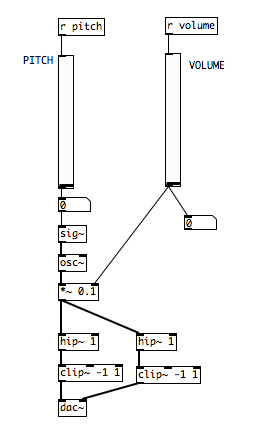
\includegraphics[width=0.3\columnwidth]{app-thereminimal-pd-patch}
	\caption{Pure Data patch used in \textit{thereminimal} application.}
	\label{fig:thereminimal-pd-patch}
\end{figure}

\begin{figure}[!ht]
	\centering
	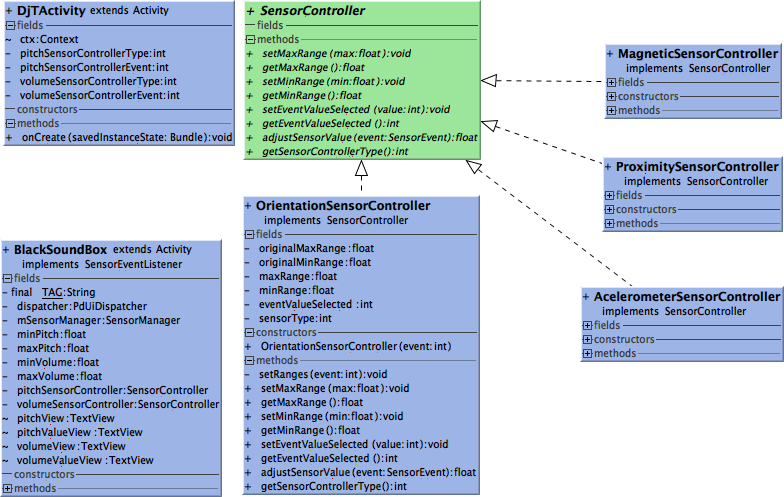
\includegraphics[width=0.9\columnwidth]{app-thereminimal-uml-classdiagram}
	\caption{UML Class Diagram of \textit{thereminimal} application.}
	\label{fig:thereminimal-uml-classdiagram}
\end{figure}

\begin{figure*}[!ht]
	\centering
	\begin{subfigure}{.30\textwidth}
		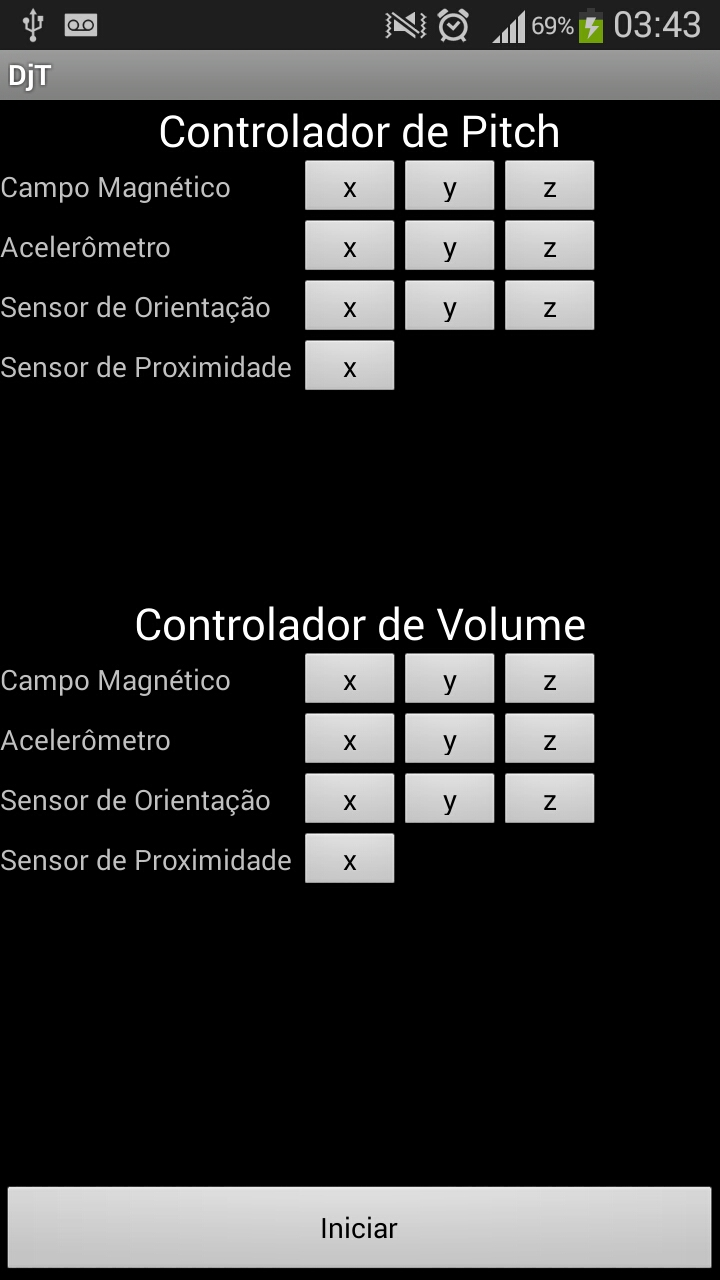
\includegraphics[width=\columnwidth]{app-thereminimal-screen1}
		\caption{First screen}
		\label{fig:appthereminimalfirstscreen}
	\end{subfigure}
	\begin{subfigure}{.30\textwidth}
		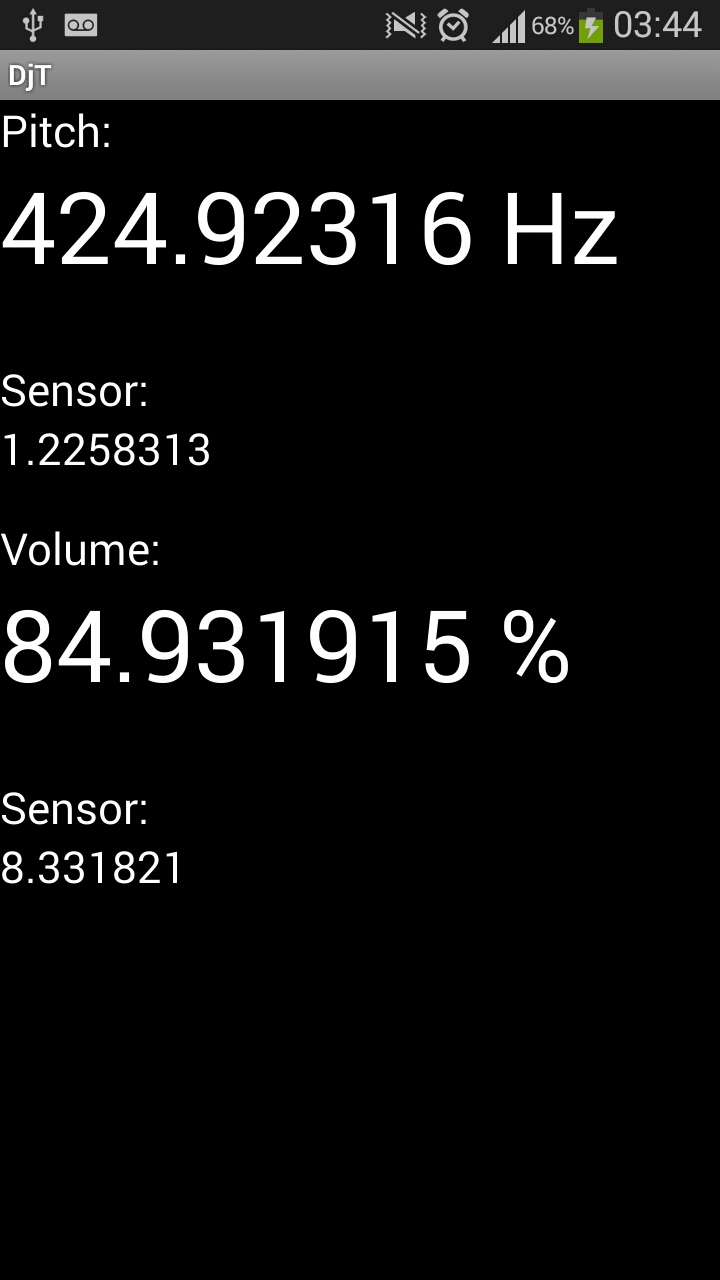
\includegraphics[width=\columnwidth]{app-thereminimal-screen2}
		\caption{Second screen}
		\label{fig:appthereminimalsecondscreen}
	\end{subfigure}
	
	\caption{Screen-shots of \textit{thereminimal} application.}
	\label{fig:appthereminimal}
\end{figure*}

The first experiences with this application provided helped on learning about the Android sensor events.
Basically, every event is captured by the API and is sent to the applications that are listening to these events depending on the predefined sample rate at application side.
The fastest sample rate option was selected for thereminimal application; this means that as soon as an event is generated, it is received by the application.

The variations in the values are too high that the changes in the frequencies are perceived as single separated notes instead of ramps or glissando.
On the other hand, the changes in the amplitude are imperceptible by most of users.

The code of the application is distributed with open source on github at the address: \url{https://github.com/deusanyjunior/thereminimal
} (visited on May, 2017).
A discussion about using libpd with Android applications was presented during a talk in the regular Compmus seminars at IME-USP on October 18, 2012~\footnote{Talk about libpd and Android: \url{http://compmus.ime.usp.br/en/node/320} (visited on May, 2017)}.

%% ------------------------------------------------------------------------- %%
\section{Java and JNI FFT on Android: Contribution to DSPBenchmarking}
\label{apesec:appdspbenchmarking}

The evaluation of audio processing on Android devices was part of the Master project conducted by the researcher Andre Bianchi at the Compmus while I was initiating my PhD research.
As soon as I learned the basics of Android application development, I started to collaborate with this project together with the researcher Max Rosan, that attended the Mobile Computing class with me.

The project evaluated many DSP methods in many Android devices focusing on the performance limits depending on the audio block size and the time required for finishing the process.
Based on the first results of this evaluation described at \cite{Bianchi2012ontheperformance}, new methods were added in order to verify the performance of some FFT variations:
traditional FFT, FFTW, multi-thread FFTW, double FFT, multi-thread double FFT.
While the FFTW is using JNI for calculating the FFTW coded in C language, the double FFT is based on the JTransforms library for parallel FFT calculation in Java language.

Although better performance was expected with these non-traditional approaches, running C/C++ code for small blocks increases the complexity of the application and also the cost for processing the same audio block.
A discussion regarding this evaluation was published as a paper at the 14th Brazilian Symposium of Computer Music~(SBCM) in 2013~\citep{deCarvalhoJunior2013fftbenchmark} and is presented in Appendix~\ref{ape:papersbcm2013}.

The multi-thread FFT had worst results than the traditional FFT, and some reasons are discussed below.
The threads were created using native thread methods available for Java language, these threads probably shared the same core of application, and in the end the threads ran concurrently.
An explanation for this behavior is that Android programming methodologies do require the use of special classes such as AsynkTask, or the packets Executor, ThreadPoolExecutor, and FutureTask.
Depending on the API and the device limitations, the threads created with these classes will provide better performance, but this information was unknown at the time of the evaluation.
Some other reasons are related to Android constraints regarding the parallelism, as the operating system decides about the threads distribution and even the activation of multi-cores.
In this case, we found out that concurrency in Android applications is a topic that requires deep discussion and turns out to be outside of the scope of this research.

The code of the application is distributed with open source on github at the address:~\url{https://github.com/andrejb/DspBenchmarking} (visited on May, 2017).

%% ------------------------------------------------------------------------- %%
\section{Android, CSound, and RoR: Touches On The Line}
\label{apesec:apptouchesontheline}

The first attempt to create collaborative applications for Mobile Music was through the use of a web service programmed using Ruby on Rails.
The idea of creating a web service was the first idea for this solution considering my personal background as web developer.
The technologies selected were based on the recent ones learned at this time.

During the period that I was Teaching Assitant for Mobile Computing course, I had to create many web services for the assignments proposed to the students and I had to choose a platform available for rapid application development~(RAD).
The Ruby on Rails~(RoR) was one of the available options at that time which caught the attention due to its simplistic way to create online solutions.
Another advantage for this solution is that the POST and GET requests using JSON format were added to the web service with few lines of code.

The CSound portability for Android devices was published on Linux Audio Conference in 2012~\citep{Yi2012csound}.
This paper inspired the use of CSound for mobile applications because it presented many examples using numerous approaches for interaction through Android inputs and CSound scores.
The \textit{MultiTouchXY}~\footnote{MultiTouchXY code: \url{https://github.com/csound/csound/blob/develop/android/CsoundAndroidExamples/src/com/csounds/examples/tests/MultiTouchXYActivity.java} (visited on May, 2017)} application was selected as a starting point for the development of \textit{Touches On The Line} application due to the high sample rate of events available from touch events.
Touch responsiveness on Android devices can have values up to 120~Hz and provides up to 10 fingers position, what implies 10 pair of position values~(x and y) on every 8~ms in the best situation~\cite{Padre2017touchresponsiveness}.

\textit{Touches On The Line} application was defined to share touch's movements online and have its path synthesized as sound.
The \textit{MultiTouchXY} demo application was provided with a CSound score that receives two values and control a sound synthesis varying frequency and timber~\footnote{MultiTouchXY score for CSound: \url{https://github.com/csound/csound/blob/develop/android/CsoundAndroidExamples/res/raw/multitouch_xy.csd} (visited on May, 2017)}.
The demo was first changed to send every new event to the web server, and to request new available values from the server all the time.
This approach was changed even during the development due to many reasons: the communication with the web server was taking too long; 
the application was getting unresponsive when too many single touch events were sent one after another, due to many processes regarding post requisitions running in background;
and the reception of too many single data (one by one) was taking too long.

The latest version of this application was developed with a buffer for a touch movement from the time the finger touches the screen to the release, including the delay between each timestamp received with the finger event.
The finger movement is synthesized in audio inside the local device by sending every single movement coordinate to the CSound synthesizer as an argument for the synthesis
The complete movement path is then sent to the web service after releasing the finger from the screen.
This data is exchanged with the web service using JSON format and contains only float numbers for position and integer numbers for delays in milliseconds.

Although this application allows many devices to participate in the same session, it was evaluated only with three devices available at lab during the period of its conception.
After its development, the application was used in some solo performances and experienced by many users during talks and presentations without problems for music interaction.
A log with all events sent through the application is available online through the main page of the web application at \url{http://wscompmus.deusanyjunior.dj/cscores} (visited on May, 2017).
An example of an event is presented below:

\begin{itemize}\itemsep0em
	\item[] [4873] [2013-10-27 11:15:27 UTC] userid: 79 - score: s 0,168750 0,181234;d1;m13 0,166667 0,181234;m17 0,166667 0,181234;m72 0,172917 0,181234;m12 0,172917 0,181234;m17 0,172917 0,181234;m17 0,172917 0,181234;u16;
\end{itemize}

This event includes the timestamp of received event, the random identification selected for the user from the application, and the score.
The score initiates with the xy initial position of the finger, includes the required delay applied before using the next finger position before each other finger position, and finishes with the delay before releasing the finger.

The development of Android applications with CSound was the topic of a talk during the regular seminars of Compmus at IME-USP, on October 1st, 2013~\footnote{Talk about Android and CSound: \url{http://compmus.ime.usp.br/en/node/377} (visited on May, 2017)}.
The application was published as a technical paper at 2nd International Conference in 2013~\citep{deCarvalhoJunior2013touches} and is presented in Appendix~\ref{ape:papericsc2013}.

%% ------------------------------------------------------------------------- %%
\section{Android and Sensors: Sensors2}
\label{apesec:appsensors2}

The creation of the \textit{thereminimal} provided the necessary code for any person with minimum knowledge about Android programming to use the Android sensors.
However, some users still found it hard to take advantage of all Android sensors in this case.
The idea of creating an Android application that could make the use of Android sensors feasible started with Sensors2Pd and extended to Sensors2OSC, resulting in the conception of Sensors2~\footnote{Sensors2 web site: \url{sensors2.org} (visited on May, 2017)} in a partnership with Thomas Mayer from Residuum.

The idea behind Sensors2 is to develop mobile applications that can help users to use Android sensors with many other technologies.
\textit{Sensors2Pd} aims the use of Android sensors with Pure Data patches that can be loaded on the application.
\textit{Sensors2OSC} sends Android sensors through the network using OSC format.
\textit{Sensors2Log} is an application that can save the sensors inputs to files inside device's internal or external memory.
The applications are being distributed through the F-Droid~\footnote{F-Droid website: \url{https://f-droid.org/} (visited on May, 2017)} platform as well as through the github.
A description of the development process of each application is present below.

%%%%%%%%
\subsection*{Sensors2Pd}
\label{apesubsec:appsensors2pd}

Many mobile applications were developed in order to turn the mobile device into an instrument just as discussed in Section~\ref{sec:mobileinstruments}.
Additionally, some applications provided the option to use Android sensors for music interaction, such as urMus, Control, and MobMuPlat.
The main restriction of these applications is that they support only few sensors, while Android sensor options are increasing through the time.
Based on this condition, \textit{Sensors2Pd} was created following an approach that is able to support all current and future Android sensors.

The idea behind \textit{Sensors2Pd} comes from the Android Sensors API~\footnote{Android Sensors API header file from repository: \url{https://android.googlesource.com/platform/hardware/libhardware/+/master/include/hardware/sensors.h} (visited on May, 2017)}.
Every type of sensor is registered at the API with an integer number.
A list of these sensors and IDs is presented at Appendix~\ref{ape:android-sensors}.
The sensor manager used on Android applications provides a listener which informs the sensor ID and the latest values from an event received by it.
Although it is possible to register to receive only the data regarding a specific sensor, the API offers the option to receive information regarding all sensors.
In this case, \textit{Sensors2Pd} provides an interface for sending the sensor's events to receivers at Pure Data patches.
The receivers inside the patches must follow the patterns:

\begin{itemize}\itemsep0em
	\item[] [receiver sensor\{ID\}v\{\#\}]
\end{itemize}

The ID represents the sensor ID from the API documentation, and the \# is the index of the event variable.
Considering the accelerometer sensor that has the ID=1 and presents 3 variables representing the x, y, and z coordinates, the user needs to add the following receivers:

\begin{itemize}\itemsep0em
	\item[]    [receiver sensor1v0]
	\item[]    [receiver sensor1v1]
	\item[]    [receiver sensor1v2]
\end{itemize}

The application was programmed to send the values in a loop.
This loop creates the messages automatically and send them based on the values that come from the API.
This approach allowed the \textit{Sensors2Pd} to be compatible with all available sensors at an Android device as long as the API continues with the same strategy.

Touch position is sent to Pure Data patches following a similar approach.
The Android system offers a listener for touches that reports the x and y position of the touch on the screen including an ID for each finger.
The IDs varies from 0 to 14, although Android devices support up to 10 touches.
A finger receives an ID as soon as it is recognized on the screen, and these IDs start with 0 increasing as new fingertips are recognized.
In case a finger is released and other fingers are still touching the screen, the next finger touching the screen will get the next available ID between 0 and 14.
The receivers used for touches follow the pattern:

\begin{itemize}\itemsep0em
	\item[]  [receiver sensorT{ID}v{\#}]
\end{itemize}

The ID represents the finger ID defined by the Android API, while the \# represents the coordinate.
An example of receivers for the finger with ID=0 are presented below:

\begin{itemize}\itemsep0em
	\item[]   [receiver sensorT0vx]
	\item[]   [receiver sensorT0vy]
\end{itemize}

Another sensor available at Sensors2Pd is the WiFi sensor.
The Android API offers a lot of information regarding all available networks, such as SSID, BSSID, frequency, and signal level in dBm.
In this case, the application sends SSID's level to Pd patches.
The user needs to configure the receiver following the pattern:

\begin{itemize}\itemsep0em
	\item[]    [receiver sensorW-{SSID}]
\end{itemize}

When the WiFi SSID is "MyRouter", the receiver needs to be:

\begin{itemize}\itemsep0em
	\item[]    [r sensorW-MyRouter]
\end{itemize}

The application was presented during the regular talks from Compmus at IME-USP on August 25th, 2014~\footnote{Talk about Sensors2Pd: \url{http://compmus.ime.usp.br/en/node/432} (visited on May, 2017)}, and its code can be found at \url{https://github.com/SensorApps/Sensors2Pd} (visited on May, 2017).
This code was also used during the development of the project Hoketus described at Section \ref{apesec:apphoketus}.
This application was published as a paper at the Joint Conference of the 40th International Computer Music Conference and 11th Sound and Music Computing Conference, Athens, Greece, in 2014~\citep{deCarvalhoJunior2014sensors2pd}.
This paper is presented at Appendix~\ref{ape:papericmc2014}.

%%%%%%%%
\subsection*{Sensors2OSC}
\label{apesubsec:appsensors2osc}

The development of \textit{Sensors2OSC} followed a strategy similar to the one applied during the development of \textit{Sensors2Pd}.
The application adapts to the available sensors at any Android device without restricting the use of new sensors that may become available.
Sensor events are converted to OSC messages and sent through UDP to a IP and Port specified by the user on the settings screen of this application.
The namespaces used for sending OSC messages have been updated for some sensors.
Table~\ref{tab:mapping} presents the current personalized OSC prefixes.
New sensors receive the prefix based on its ID. For instance, a new sensor with ID=30 will receive the prefix /30.

\begin{table}[t]
	\centering
	\caption{Mapping from Android sensors to OSC messages in Sensors2OSC}
	\label{tab:mapping}
	\begin{tabular}{|l|l|l|}  \hline
		ID & OSC prefix                  & Dimensions \\   \hline
		1  & \lstinline$accelerometer$             & 3          \\
		2  & \lstinline$magneticfield$             & 3          \\
		3  & \lstinline$orientation$              & 3          \\
		4  & \lstinline$gyroscope$                 & 3          \\
		5  & \lstinline$light$                      & 1          \\
		6  & \lstinline$pressure$                   & 1          \\
		7  & \lstinline$temperature$                & 1          \\
		8  & \lstinline$proximity$                  & 1          \\
		9  & \lstinline$gravity$                   & 3          \\
		10 & \lstinline$linearacceleration$        & 3          \\
		11 & \lstinline$rotationvector$            & 4          \\
		12 & \lstinline$relativehumidity$           & 1          \\
		13 & \lstinline$ambienttemperature$         & 1          \\
		14 & \lstinline$magneticfielduncalibrated$  & 6          \\
		15 & \lstinline$gamerotationvector$        & 3          \\
		16 & \lstinline$gyroscopeuncalibrated$     & 6          \\
		17 & \lstinline$significantmotion$          & 1          \\
		18 & \lstinline$stepdetector$               & 1          \\
		19 & \lstinline$stepcounter$                & 1          \\
		20 & \lstinline$georotationvector$         & 4          \\
		21 & \lstinline$heartrate$                  & 1         \\ 
		22 & \lstinline$tiltdetector$               & 1      \\
		23 & \lstinline$wakegesture$             & 1      \\
		24 & \lstinline$glancegesture$           & 1      \\
		25 & \lstinline$pickupgesture$           & 1     \\ \hline
	\end{tabular}
\end{table}

The first design of \textit{Sensors2OSC} had the option to select the coordinates of each sensor that would be sent through OSC, as presented in Figure~\ref{fig:appsensors2oscfirstdesign}.
In this case, one OSC message would be sent for every coordinate selected.
As the UDP messages are received out of the expected sequence, some coordinates of a punctual sample can be lost even on local networks.
This condition led to an update on the application in which the user selects only the sensor instead of its coordinates, and all coordinates are sent in a single bundle.
The current version of \textit{Sensors2OSC} packs all values and send them in a single OSC message, and its design is presented in Figure~\ref{fig:appsensors2oscseconddesign}.

\begin{figure*}[!ht]
	\centering
	\begin{subfigure}{.30\textwidth}
		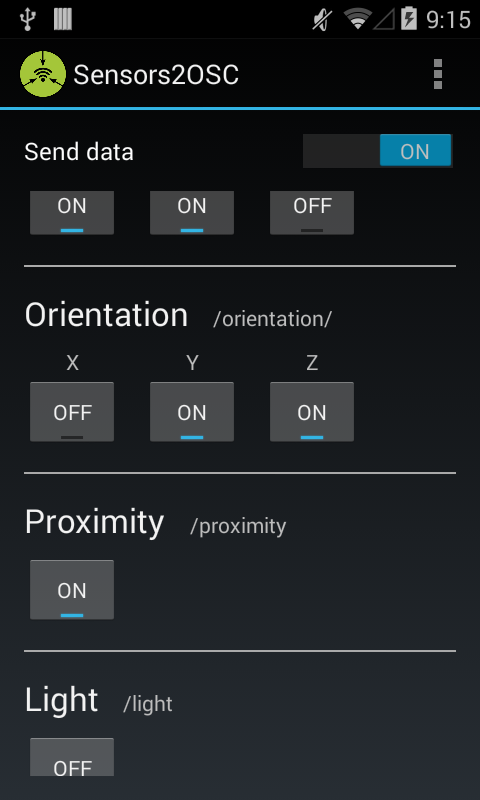
\includegraphics[width=\columnwidth]{osc_main}
		\caption{First screen design}
		\label{fig:appsensors2oscfirstdesign}
	\end{subfigure}
	\begin{subfigure}{.28\textwidth}
		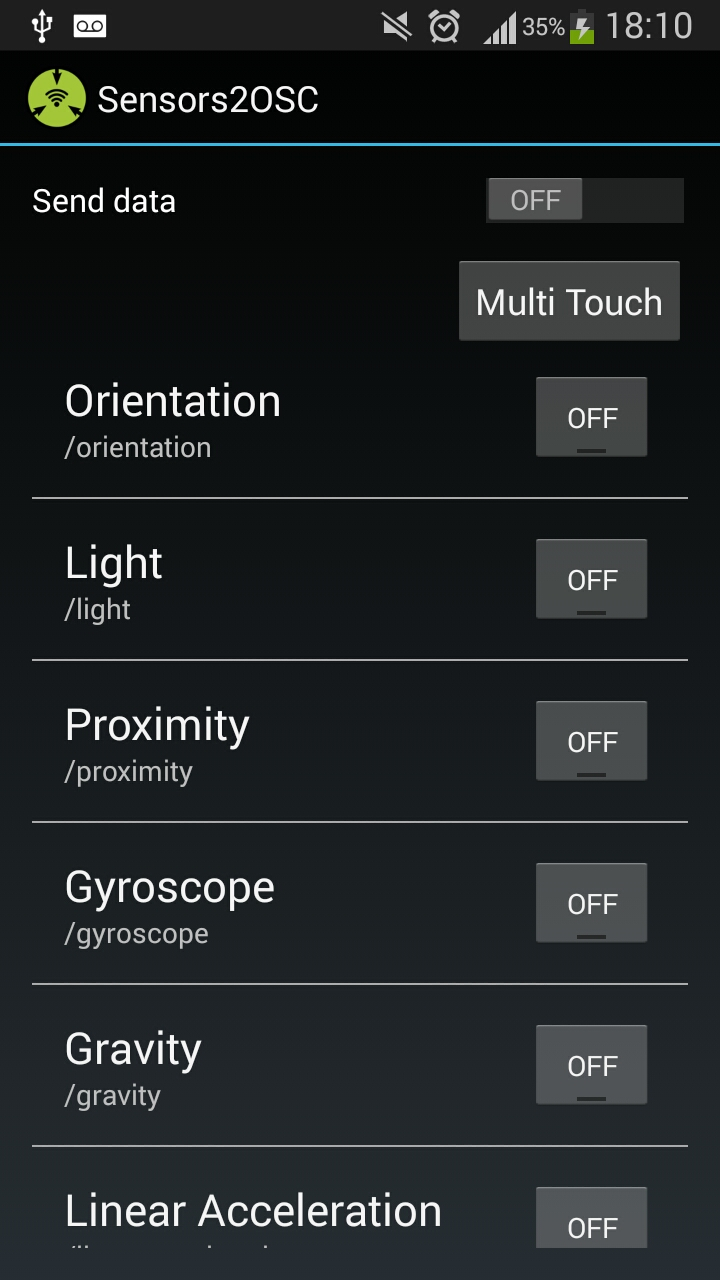
\includegraphics[width=\columnwidth]{osc_main_new}
		\caption{Current design}
		\label{fig:appsensors2oscseconddesign}
	\end{subfigure}
	
	\caption{Screen-shots of \textit{Sensors2OSC} main screen designs.}
	\label{fig:sensors2oscmainscreen}
\end{figure*}

The application has been used by Thomas Mayer in many of his performances, and I used this application in the performance \textit{AntonioZ} at \textit{Concertos de Computação Musical}~(Computer Music Concerts)~\footnote{Concerts description: \url{https://theantonioz.wordpress.com/} (visited on November, 2018)} organized by me in 2016 at the IME-USP during \textit{Semana de Arte e Cultura da USP}~(Art and Culture Week from USP).
Other users have reported the use of this application and requested modifications.
Mladen Radolovic is a Croatian user that requested the addition of an option to send NFC tags' information through OSC and now the application is able to send the NFC tags identification through the namespace /nfc.
Tal Kirshboim is a German user that included the Multitouch option on the application and continue debugging the code.
A user from Japan also contributed with the translation of the application to Japanese, and now the application is internationalized to four languages including English, German, and Portuguese.

A discussion about mapping Android sensors using OSC on Android devices with this application was presented during a talk in the regular Compmus seminars at IME-USP on June 29th, 2015~\footnote{Talk about mapping Android sensors to OSC: \url{http://compmus.ime.usp.br/en/node/465} (visited on May, 2017)}.
The application code can be found at \url{https://github.com/SensorApps/Sensors2OSC} (visited on May, 2017).
This application was published as paper at the Sound and Music Computing Conference at Maynooth, Ireland, in 2015~\citep{deCarvalhoJunior2015sensors2osc}.
This paper is presented at Appendix~\ref{ape:papersmc2015}.

%%%%%%%%
\subsection*{Sensors2Log}
\label{apesubsec:appsensors2log}

During the experiences with these applications I was invited to work in a project related to patient monitoring. % paciente de que? apneia?
The main goal of this project was to diagnose a person's health by analyzing the data registered while he/she is sleeping
The code of Sensors2Pd was then changed to record the sensors values to files instead of sending to Pure Data patches.
Another feature of this project was the audio recording into MP3 and WAVE formats.

The current application is still under development, but it has been tested in many different situations.
The first evaluation was for monitoring a patient in \textit{Laboratório do Sono}~(Sleep Lab) at \textit{Instituto do Coração}~(Heart Institute) from USP.
A strap was designed to hold the mobile device over the body of a patient and allow the device to be in the same position of the patient.
Audio and sensors were registered during a whole night of sleeping.
The data was then retrieved from the mobile device through the internal memory using the USB cable and evaluated by many programs on Desktop computers.
Other evaluations were conducted to register the sensor values and verify movements accuracy with success.
The use of this application generated many interesting results regarding Android sensors.
Although the application recorded data for more than 10~hours in a row, the battery consumption was less than 50~\% in a Sony Xperia Play smartphone with the screen turned off during the evaluation.

After the experiments, the application was dubbed \textit{Sensors2Log} and aggregated to the \textit{Sensors2} collection.
The application can be used in many monitoring process with options for selecting the sensors and the audio recording settings.
Figure~\ref{fig:sensors2log} shows two screens of the application and the current application code can be found at \url{https://github.com/SensorApps/Sensors2Log} (visited on May, 2017).

\begin{figure*}[!ht]
	\centering
	\begin{subfigure}{.35\textwidth}
		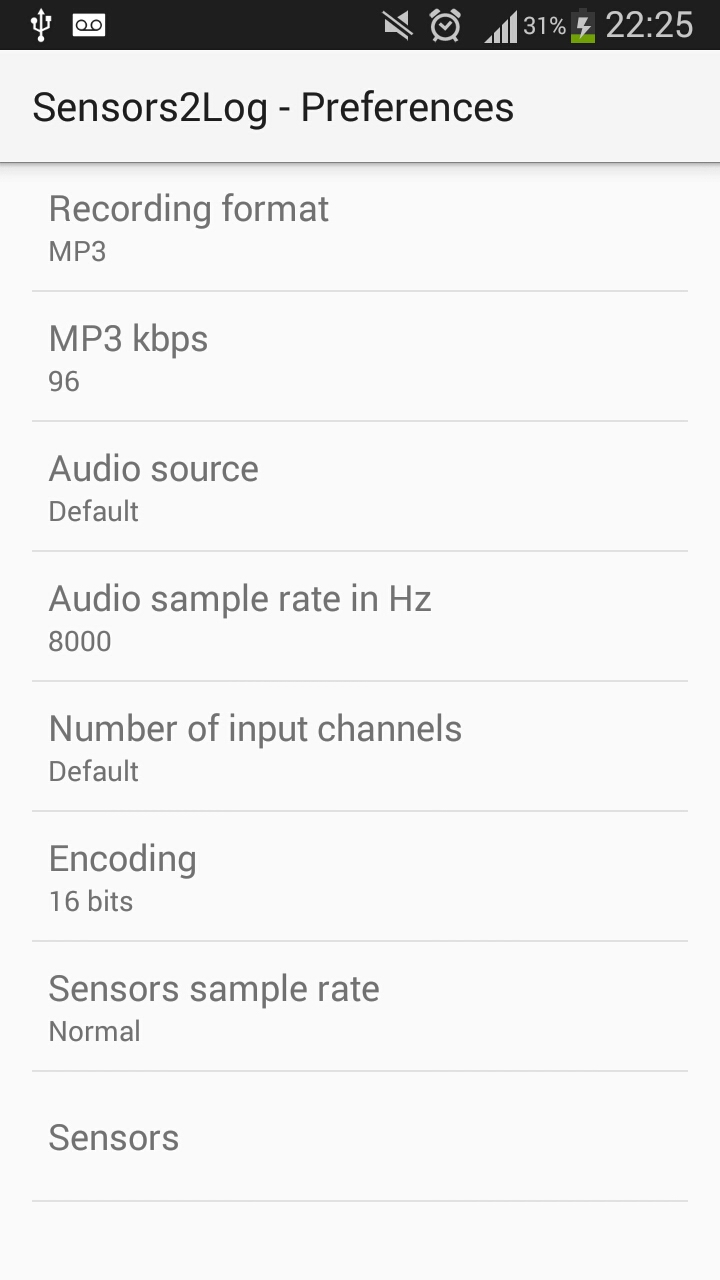
\includegraphics[width=\columnwidth]{sensors2log_screenshot1}
		\caption{Preferences screen}
		\label{fig:appsensors2log1}
	\end{subfigure}
	\begin{subfigure}{.35\textwidth}
		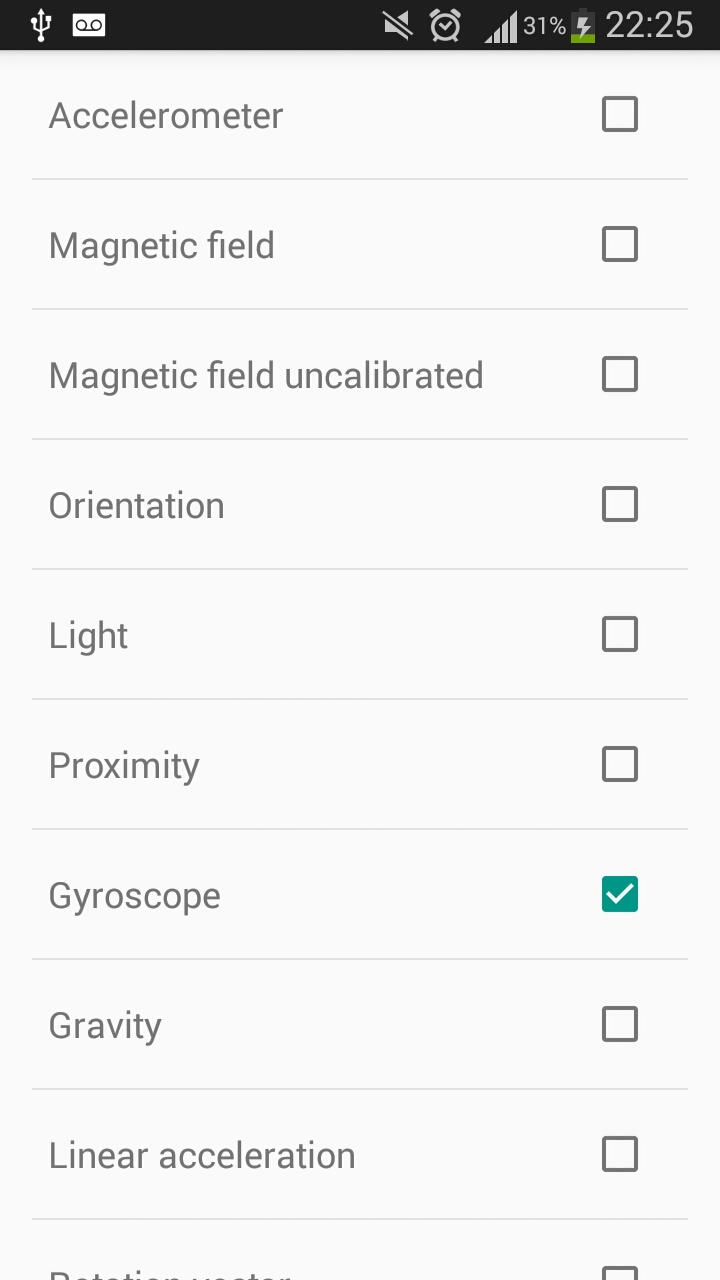
\includegraphics[width=\columnwidth]{sensors2log_screenshot2}
		\caption{Sensor selection screen}
		\label{fig:appsensors2log2}
	\end{subfigure}
	
	\caption{Screen-shots of \textit{Sensors2Log}.}
	\label{fig:sensors2log}
\end{figure*}

%% ------------------------------------------------------------------------- %%
\section{Indoor localization and Pure Data: Hoketus installation}
\label{apesec:apphoketus}

The code of \textit{Sensors2Pd} was used to create the application \textit{Hoketus} during an installation under the same name.
This installation took advantage of the WiFi level to identify users close to specific routers.
The application was created with the Sensors2Pd code embedded and the application interface was personalized especially for this installation. 

Some smartphones were configured as hotspots and the Pure Data patches created for this installation were defined to synthesize different sounds depending on the SSID found.
The participants were invited to install an application that would find hotspots and also synthesize different sounds.
A web server was set up using the same technologies and approaches presented in Section~\ref{apesec:apptouchesontheline} but with specific pages for each hotspot.
The participants' application had a method to send the level of the SSID found to the web service, and the hotspots' application were configured to request the SSIDs' level in order to amplify their synthesis depending on the number of close devices.

During the performance, the hotspots used the 3G interface to connect to the Internet, since the Wi-Fi interface was being used as a hotspot antenna. 
It is important to notice that the participants were possibly using the 3G data connection and nobody reported any issue regarding the consumption of the 3G plan during the performance.
Most of the questions regarding the installation were related to interaction aspects that were somewhat incomprehensible at some locations.
The Figure \ref{fig:installation} represents the installation with the hotspots and the participants while Figure \ref{fig:installation-schema} shows an example of network communication between the mobile devices. 
In both images the hotspots have a circle representing their best signal strength area.

\begin{figure*}[!ht]
	\centering
	\begin{subfigure}{.45\textwidth}
		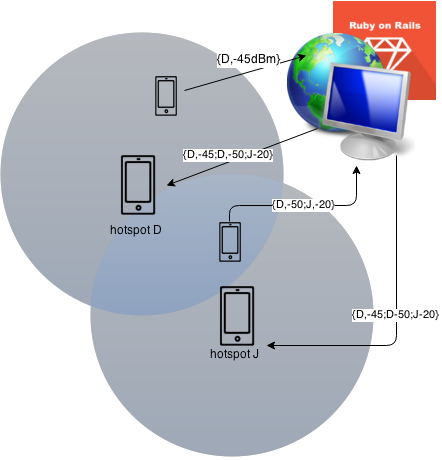
\includegraphics[width=.90\columnwidth]{nime2015-schema}
		\caption{Network communication}
		\label{fig:installation-schema}
	\end{subfigure}
	\begin{subfigure}{.45\textwidth}
		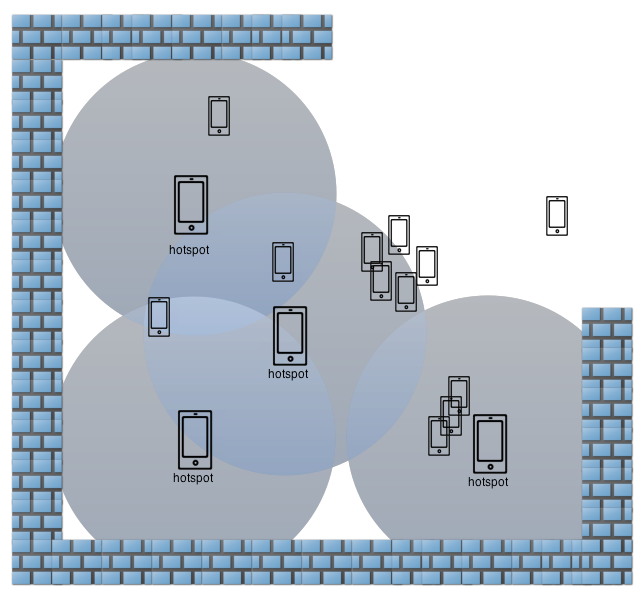
\includegraphics[width=\columnwidth]{nime2015-installation}
		\caption{Four hotspots installation}
		\label{fig:installation}
	\end{subfigure}
	
	\caption{Hoketus installation.}
	\label{fig:hoketusinstallation}
\end{figure*}

An aesthetic discussion about this installation and other experiences with Sensors2PD can be found at the paper presented at The Fourteenth Biennial Symposium on Arts and Technology, Connecticut College, New London, CT, USA, in 2014~\citep{Bandeira2014notes}.
A discussion about the advantage of using WiFi for indoor localization with this application during the Hoketus project was published as a paper and presented as a poster during at the International Conference on New Interfaces for Musical Expression, Baton Rouge, Lousianna, USA, in 2015~\citep{deCarvalhoJunior2015indoor}.
These papers are presented at Appendix~\ref{ape:paperbats2014} and Appendix~\ref{ape:papernime2015}, respectively.
The code used on \textit{Hoketus} mobile application is available at \url{https://github.com/deusanyjunior/hoketus} (visited on May, 2017).

%% ------------------------------------------------------------------------- %%
\section{Cloud Services for presentations: pubslides}
\label{apesec:apppubslides}

One of the first simple and useful application created with the use of Cloud Services during this research was the \textit{pubslides}.
This application was made with HTML, CSS, and Javascript with the aim of sharing the current slide page with the audience during a presentation.
The person that is giving a talk can control the current slide position from the master page of \textit{pubslides}, while the other users follow the presentation on the client page.

The process for adapting any presentation to this application is also simple.
The \textit{pubslides} code needs to be available at some web server accessible by the audience from the Internet, the presenter needs to open the master page presented on Figure~\ref{fig:pubslidesmaster}, and the the audience needs to open the index page presented on Figure~\ref{fig:pubslidesclient}.
The current version of pubslides require the PDF to be converted to SVG files through a bash script.
Every page of the PDF is then converted to an image, and this image is projected as the background image of a page at audience's screen.

The application is compatible with any device that has a browser, including smartphones.
The communication between the master and clients takes advantage of PubNub cloud service.
This cloud service was selected after some evaluations against Pusher cloud service.
This comparison is better presented at the Chapter~\ref{cap:evaluations}, but the main point considered was that PubNub offers a low packet lost rate even on free plans.

\begin{figure*}[!ht]
	\centering
	\begin{subfigure}{.45\textwidth}
		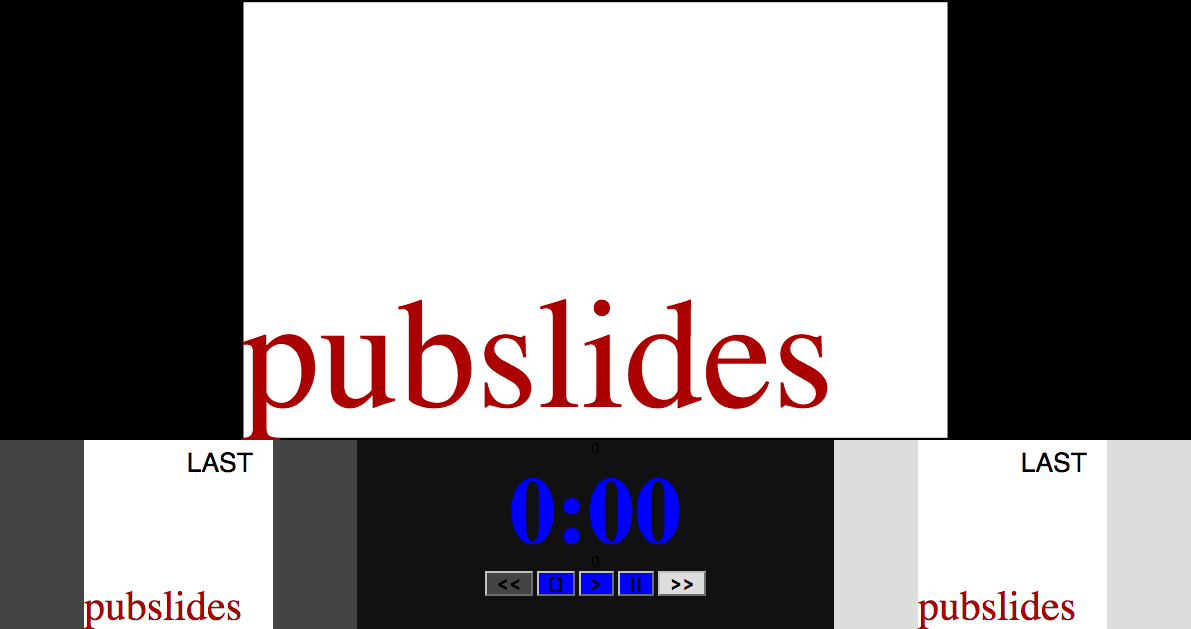
\includegraphics[width=\columnwidth]{pubslides_master}
		\caption{Master page}
		\label{fig:pubslidesmaster}
	\end{subfigure}
	\begin{subfigure}{.45\textwidth}
		
\includegraphics[width=\columnwidth]{pubslides_client}
		\caption{Client page}
		\label{fig:pubslidesclient}
	\end{subfigure}
	
	\caption{pubslides application pages.}
	\label{fig:pubslidesapplication}
\end{figure*}


This application is currently used at the \textit{TV CompMus} page~\footnote{TV CompMus page: \url{http://compmus.ime.usp.br/en/tv} (visited on May, 2017)} used during the regular talks of the Compmus group.
The code of the application is available at \url{https://github.com/deusanyjunior/pubslides} (visited on May, 2017).

%% ------------------------------------------------------------------------- %%
\section{Cloud Services and SuperCollider: SuperCopair}
\label{apesec:appsupercopair}

The conception of \textit{SuperCopair} application happened during the period while I was an exchange student at University of Michigan.
I was interacting the live coder Sang Won Lee and noticed that few solutions are available for a distributed collaborative live coding.
After some research we discussed solutions and alternatives with Georg Essl and a the application presented in this section came out.

The \textit{SuperCopair} application was created as a package to the Atom.io~\footnote{Atom.io website: \url{http://atom.io} (visited on May, 2017)} IDE.
Defined as 'a hackable text editor for the 21st Century' on its site, Atom is a text editor created using web technologies and has its development powered by the github community.
This IDE has numerous packages for many programming languages and presents some solutions for coding, debugging, and managing projects.
Atom packages are programmed in CoffeeScript~\footnote{CoffeeScript website: \url{coffeescript.org} (visited on May, 2017)}, which is a programming language that can easily be converted to Javascript and can also integrate its libraries.
The developers can install Atom packages to enable various functionalities in the IDE such as: communicate through chats, use auto-complete in certain programming language syntax, interact with desktop and web applications, integrate with the terminal command line, and have many options based on other packages.
These features have motivated the development of SuperCopair package for Atom.

SuperCopair is based on two Atom packages: atom-supercollider and atom-pair.
The first package turns Atom.io as an alternative SuperCollider IDE and permits users to openly communicate locally with SuperCollider audio server through OSC in the same way we can do on SC-IDE.
Moreover, the users can take advantage of other Atom packages additionally to quarks packages.
The latter package is used for pair programing through the Internet.
The atom-pair package is based on Pusher cloud service and its default configuration is based on the community free plan, but a user can modify the settings and use the user’s own keys within the personal free or paid plan. 
We decided to merge both packages to add new features for collaborative live coding, and finally had dubbed it the SuperCopair package.
The main idea is that all participants have the opportunity to evolve into a collaborative performance.

The IDEs for SuperCollider have, by default, shortcuts to evaluate a line, a block, and to stop all sound process that is running.
In addition to these options, the SuperCopair package includes methods and shortcuts to broadcast these events and execute them on all users connected at the same pairing session.
Through the shortcuts, one can decide to evaluate selected code either only in the local machine, or in all computers of the session.
One can also turn on a broadcast alert option in the settings in order to be asked before evaluating every broadcast event sent by another user in the same session. 
This allows each individual to have control over which portion of code can be evaluated in the local machine.
The broadcast events are diffused through the cloud service and are expected to be evaluated as soon as each device receives the event message.

Networked live coding environments have been focused in collaboration.
All participants are working together to execute a musical piece and share the same final result as a common goal.
In most of the cases, sound is the only artifact that is shared, but the performers can also share codes.
Some tools enable chatting, audio, and video interaction between the participants, whether they are sharing the same physical space or they are in different locations.
Although the experiments with SuperCopair have been conducted as distributed collaborative live coding sessions, the cooperative environment has emerged during some moments.

During the sessions using SuperCopair, we had participants from different levels of experience on live coding and also some new users that decided to learn how to code during the session.
The collaboration on the final sound was similar to other live coding sessions, but the experience added another way of interaction in live coding: the cooperation. 

The cooperation aspect emerged from some events that came into view from the live coding sessions.
Experienced users are faster and have written lots of code from the scratch without any problem, while the apprentices start from basic structures or from portions of codes available on the file.
As all users were trying to synthesize the codes on all computers, it became easy to perceive if something was going wrong because everybody was sharing the code, evaluation, synthesis, and errors.
The errors coming from novice programmers were often fixed by the experienced users, and they also discussed the solutions between themselves using comments on the file.
Some tricks from the live coding practice were introduced by advanced users and the initial learners rapidly became instructors for new users and these instructors were following the same cooperative practices of the experienced users.
These events are examples of how this application can be used in many different ways: for collaborative and also cooperative performances.

A discussion about the use of cloud services for designing collaborative applications was presented during a talk in the regular Compmus seminars at IME-USP on April 6th, 2015~\footnote{Talk about cloud services: \url{http://compmus.ime.usp.br/en/node/461} (visited on May, 2017)}, and the discussion about the use of SuperCopair for live coding was presented August 19th, 2015~\footnote{Talk about SuperCopair: \url{http://compmus.ime.usp.br/en/node/469} (visited on May, 2017)}.
The code of this application is available at \url{https://atom.io/packages/supercopair} (visited on May, 2017) with the documentation and environment setup instructions.
The application was published as a paper at International Conference on Live Coding, Leeds, West Yorkshire, UK, in 2015~\citep{deCarvalhoJunior2015supercopair}, which is presented at Appendix~\ref{ape:papericlc2015}.
A discussion about using SuperCopair for cooperative live coding was published at Simposio Latinoamericano de Informática y Sociedad from the XLI Conferencia Latinoamericana en Informática (CLEI), Arequipa, Peru, in 2015~\citep{deCarvalhoJunior2015cooperative}, and is presented at Appendix~\ref{ape:paperclei2015}.

%% ------------------------------------------------------------------------- %%
\section{Cloud Services and Web Audio: Crowd in C[loud] piece}
\label{apesec:appcrowdincloud}

An application for collaborative performance using smartphones was created with Sang Won Lee and Georg Essl while I was doing research at University of Michigan.
The main idea behind this application is that it is fully deployed on the web, the communication between devices is conducted through cloud services, and the audio synthesis is made with Web Audio API.
This combination allowed participants to join the performance using any device and any kind of Internet connection as there was small messages transmission instead of audio.

As the name of the piece suggests, the crowd (audience) plays the musical instrument in C Major. 
This is directly inspired from the piece \textit{In C}, by Terry Riley~\citep{Riley1964inc}. 
In this piece, musicians (with various instruments) were guided to play pre-composed melodic fragments in sequence for a random amount of time. 
As it is up to each musician to decide how many times to play one fragment, the collective outcome of the ensemble creates a heterophonic texture of chance.
Similarly, in \textit{Crowd in C[loud]}, each audience member plays a series of short snippets composed by himself/herself and by other audience members.
The interface provided will first guide a participant to compose a short \texttt{``tune''} that has five musical notes in C major.

Once the participant finishes the composition, he or she can browse, and play, what other audience members have composed. 
It is thus quite similar to Terry Riley's \textit{In C}, in that one determines for oneself how long to play a tune. 
The difference is that there is no pre-composed fragments but each audience member will contribute to the piece by submitting a short melody.
In this way, participants will have their own tunes and a chord scale become the common ground upon which the entire audience plays. 
In addition, there is a separate musician performing the piece on stage at the same time with the audience members in \textit{Crowd in C[loud]}.
The role of the musician is to be a meta-performer who can control the chord scale in which the audience members are playing.
For example, the meta performer can, on the fly, change the instrument tuned in C major scale to a different chord scale (e.g., C Minor, Pentatonic Scale). 
This performer only controls the harmonic flow of the piece as generated by the crowd.
The interplay between the musician and audience members ensures that each audience member will play individual patterns while a musician can progress the piece by changing chord scales. 
This performer-audience pairing model comes from a previous work of \textit{echobo}~\citep{Lee2013echobo} where audience members played a simplified key instrument on smartphones with the chord progression determined by a performer on stage and synchronized over a mobile network.

The performance structure was inspired by other networked pieces that presented a centralized network with a server for receiving and sending information~\citep{Weinberg2005interconnected}.
However, our choice of using the Pub Nub cloud service set us free from the burden of developing a custom server application, which is replaced with a single web page written in HTML and Javascript.
This will be a useful setup for artists without networking background that want to write a network music piece with an interactive web page.
PubNub cloud service permits easy interconnection between users through channels using publish-subscribe (or pub-sub paradigm).
An application~(or device) can subscribe to a channel and receive every notification that is published to the channel. 
For example to broadcast a message to all devices, a device can publish a message to a channel that every device is subscribed to. 
This provides a convenient abstraction that is robust against changes in network or end-user device and allows dynamic reconfiguration of participation.
The push(or publish) notifications paradigm also makes performances more robust against technical disruptions such as disconnection and delays.

The left side of Figure \ref{fig:performance} presents the performance setup at the concert hall.
There are two kinds of web pages running during the performance, one for the performer and another for the audience.
The performer seat center-stage and his application (a web page) is projected onto a screen for the participants seated in the audience.
The audience is instructed to visit the application that has the musical instrument on.
The performance hall has wireless network available from the university and has a good reception of mobile network connectivity such as 3G.

A representation of the cloud service with the channels is on the right side of the Figure~\ref{fig:performance}.
For this application there are three types of channels following the PubNub API for web application: a performer channel, an audience channel and individual channels equaling the participant number. 
The performer application is subscribed to the performer channel to receive messages sent from audience member's devices. 
Once a participant visits, it requests a performer's application to create an individual channel by publishing a message to the performer channel.
The individual channel is then created to respond to an audience application's request, typically for the audience to retrieve a tune composed by others.
When the page is loaded, every device is given a universal unique identifier (UUID) from the cloud service API, which is used to create an individual channel.
Lastly, all the audience members are subscribed to the audience channel. 
This channel is used for crowd control: to send textual instructions, to live-code the mobile instrument, to start/end the performance and to troubleshoot the performance when it goes wrong (silence, refreshing the page).

\begin{figure}[t]
	\centering
	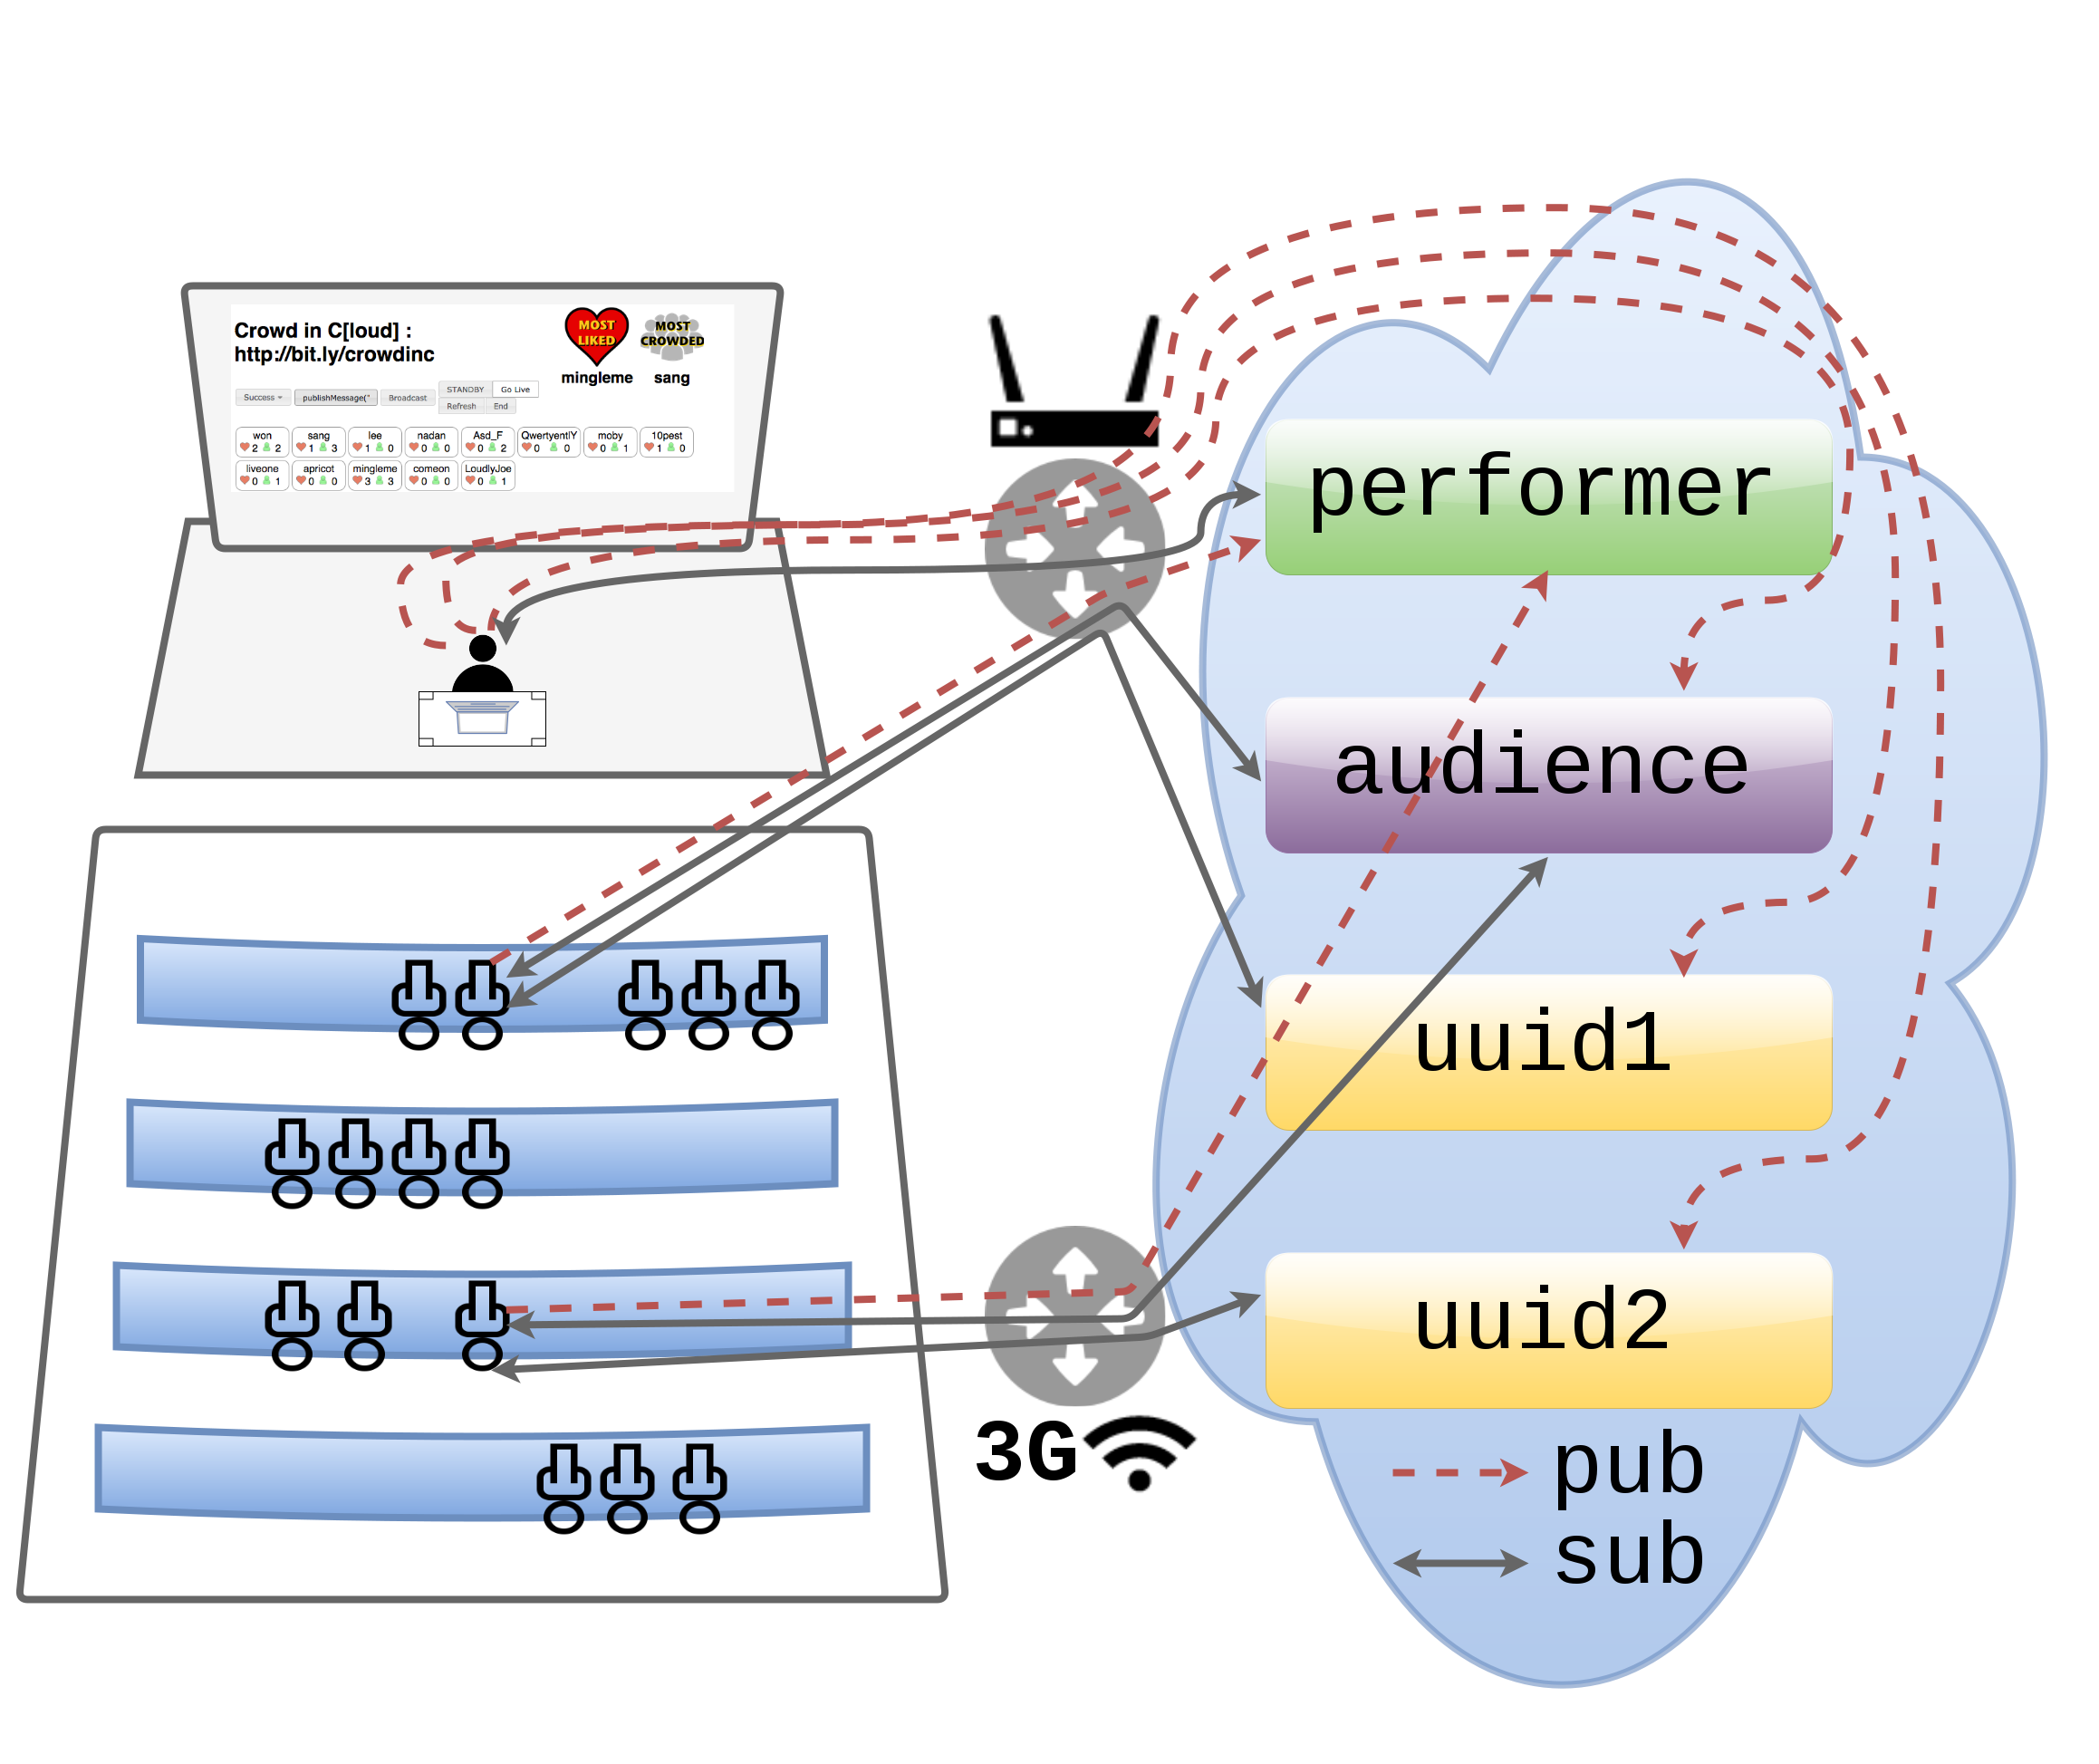
\includegraphics[width=0.5\columnwidth]{performance}
	\caption{Performance structure. The left side depicts the performance space. On the right side, a rectangle represent a channel, solid lines show publishing and dotted lines show subscription.}
	\label{fig:performance}
\end{figure}

\textit{Crowd in C[loud]} was performed at many venues during the past two years and the debut happened on April 18, 2015 in Stamps Auditorium at the Walgreen Drama Center on the U-M North Campus~\footnote{Debut of \textit{Crowd in C[loud]}: \url{http://www.eecs.umich.edu/eecs/about/articles/2015/w15-mobile-phone-ensemble-performance.html} (visited on May, 2017)}.
The video from the debut is available at \url{https://www.youtube.com/watch?v=8RWgXoM2BCA} (visited on May, 2017) and a multi-camera video of a performance in Atlanta is available at ~\url{https://www.youtube.com/watch?v=8nnrKJ4Ap0c} (visited on May, 2017).

The discussion about sound synthesis was published as a paper in 2nd Web Audio Conference (WAC), Atlanta, Georgia,  USA, in 2016~\citep{Lee2016crowd} and the discussion regarding network communication through the cloud services was published in the 16h International Conference of New Instruments for Musical Expression, Brisbane, Australia, in 2016~\citep{deCarvalhoJunior2016understanding}.
The papers published in these conferences are presented in Appendix~\ref{ape:paperwac2016} and Appendix~\ref{ape:papernime2016}, respectively.
A discussion about the application was presented during a talk in the regular Compmus seminars at IME-USP on September 16th, 2015~\footnote{Talk about Crowd in C[loud]: \url{http://compmus.ime.usp.br/en/node/475} (visited on May, 2017)}
The code used on the application is available at \url{https://github.com/panavrin/tindermusic} (visited on May, 2017), with a live demo for the performer at \url{https://crowdinc.github.io/performer} (visited on November, 2018) and for the audience at \url{https://crowdinc.github.io} (visited on November, 2018).

%% ------------------------------------------------------------------------- %%
\section{iOS, Lua, and Network communication: Performances with urMus}
\label{apesec:appsumich}

The final projects of the course audited at University of Michigan resulted in musical performances.
One of the performances that I participated during the conception was \textit{Crowd in C[loud]} presented in Section~\ref{apesec:appcrowdincloud}.
Two other performances described below were based on mobile applications created using the \textit{urMus} platform.
Both performances used a similar approach regarding the network communication inside the platform using the Lua language.

Although the \textit{urMus} supports OSC, listening to OSC messages through a specific IP is unavailable so then the Multicast communication was discarded.
The technology used in this case was the ZeroConf and Bonjour methods for network advertising and discovery.
A Lua code simulating Multicast for urMus is presented and commented at Listing~\ref{urMusLuaMulticast}.
In a brief, the master device was configured to discover all other devices advertisements.
Every discovered device is attached to a list of available devices.
The master device can use this list to send messages to all devices.

\begin{footnotesize}
	\lstset{language=Java, caption=Example of Lua code used at urMus platform for Multicasting in LAN, captionpos=b, label=urMusLuaMulticast, numbers=none, numberstyle=\scriptsize}
	\begin{lstlisting}[frame=single]
	friends = {} -- List with IPs from friends
	friendsKey = {} -- List that associates the latest byte from friend's IP with its index at friends list
	
	local myIP, myPort = HTTPServer()
	
	-- The latestDot is the index before the latest byte from an IP.
	latestDot = string.find(myIP, '.', 
	string.find(myIP,'.',
	string.find(myIP, '.', 1 , true)+1, true)+1, true)
	
	-- The id will be the latest byte from the IP
	local ownId = tonumber(string.sub(myIP, latestDot+1))
	
	-- Call this function when a device joins the performance
	local function NewConnection(self, name)
	DPrint("new friend "..name)
	DPrint("")
	for j,u in pairs(friends) do
	if u == name then
	return
	end
	end
	friendLatestDot = string.find(name, '.', string.find(name, '.',string.find(name, '.',1, true)+1, true)+1, true)
	friendId = tonumber(string.sub(name, friendLatestDot+1))
	table.insert(friends, name) -- Adds IPs to the list friends
	friendsKey[friendId] = table.getn(friends) -- Sets the IP index to the lates byte
	end
	
	-- Call this function when a device leaves the performance
	local function LostConnection(self, name)
	for l,w in pairs(friends) do
	if w == name then
	table.remove(friends,l)
	end
	end
	end
	
	-- Call this function to send a message to every participant device
	function sendNote(noteToSend)
	DPrint("sent "..noteToSend)
	DPrint("")
	-- Send the message to every device on the list
	for indexIp = 1, table.getn(friends) do
	local ip = friends[indexIp]
	SendOSCMessage(ip,8888,"/urMus/numbers",noteToSend, ownId, currentPage)
	end
	end
	
	-- Call this function when a packet is received from network
	function gotOSC(self, noteReceived, senderId, senderPage)
	DPrint("got osc")
	DPrint("")
	...
	end
	end
	
	-- Call these functions when a friend joins or leaves the network
	bg:Handle("OnNetConnect", NewConnection)
	bg:Handle("OnNetDisconnect", LostConnection)
	
	-- Listen and receive messages in the same Bonjour group
	StartNetAdvertise("ttss",8889)
	StartNetDiscovery("ttss")
	
	-- Call this function for every OSC message received
	bg:Handle("OnOSCMessage",gotOSC)
	
	SetOSCPort(8888)
	host, port = StartOSCListener()
	\end{lstlisting}
\end{footnotesize}

This approach was evaluated for different numbers of devices and the more devices we added the more the application was overloaded with the network communication.
The problem happens due to the loop throughout the list of IPs for every message occur inside the device instead of a loop at the router.

The pieces using this code are described in the next sections.
The performances were performed on April 18, 2015 in Stamps Auditorium at the Walgreen Drama Center on the U-M North Campus~\footnote{Infomation about performances with urMus in 2015: \url{http://www.eecs.umich.edu/eecs/about/articles/2015/w15-mobile-phone-ensemble-performance.html} (visited on May, 2017)}.
The videos from these performances are available at \url{https://www.youtube.com/playlist?list=PLcDYUKIkEOpZ9qMRzlfEg2ziEeJxBG4dF} (visited on May, 2017).

%%%%%%%%
\subsection*{Twinkle, Twinkle Smartphone Star}

This performance was conceived in a partnership with Zachary Boulanger and the concept is related to playing with the idea of expectations. 
The master performer would be a composer using the master application with an 8-key keyboard that was configured to send every key touched to all the friends available.
The other performers would have the same keyboard and they would receive the information regarding the notes to be played.
Each note was converted to falling balls over the keyboard keys and the performers were invited to touch the correspondent key as soon as the ball reaches the other side of the screen.

On the performance conception, the composer expects the performers to play his creation exactly right, however the players soon realize they are unbound to this.
The audience expects to hear well-known canons and to hear the music ``written'' by the composer, but once the performers start changing it up these expectations are broken.
While composer is creating melodies based on canons, the audience will see the notes coming from the top of the projector screen and they are expected to hear the notes once they reach the bottom. 
In the beginning the performers will play only their specific notes, but some of them are going to try other notes and the perception of the melodies will diverge from the reality. 
As the performers decide to walk on the stage, it will became hard to know who is expected to play the right note.

The audience will expect some control from composer hands, but he is using a headphone and he is acting like a deaf composer. 
In the middle the composer will take out the headphone, he will try to control the performers again, and stop sending notes to the end of the piece.
The sound experience comes from the idea that the audience will expect some melodies based on the notes that are falling down, and the players will play the notes at their own pace, without knowing the melody composed by the composer.

The code used for the performance is available at \url{https://github.com/deusanyjunior/ttss} (visited on November, 2018).

%%%%%%%%
\subsection*{Himalayan Singing Bowl}

Biqiao ``Didi'' Zhang was the composer of this piece and I participated with Zachary Boulanger as partners during the development of the mobile application.
In this piece we simulate a himalayan singing bowl through multiple mobile devices. 
One person is the ``conductor''/``leader'' of the performance and this person controls which note the devices are playing (e.g. C3) and how people should be moving their devices. 
Ideally, only the performers know who the leader is.
The performers will all be standing in a circle on stage, facing inward. 
They move their devices up and down to control the volume and left and right to control the ``beating'' of the sound. 
The color on their screen changes with their movement. 
A projector displays a video of a singing bowl, so the audience knows what the performance is based on.

The difference in frequencies by each performer, their place on the stage, and the changing color of the screen mimicking their movements all provide a unique spatial element to the performance. 
The absence of a clearly defined conductor also lends to the idea of circular performance with everyone following everyone else’s movements and actions. 
This shows that the performance not only simulates the singing bowls musically, but in a physical aspect as well.
The sound is simulating an actual singing bowl, with the performers forming the bowl itself. 
Each person has a different frequency than those next to them, giving a spatial element to the musical experience. 
The performance is then made more musically interesting with the addition of different pitches, dynamics, and ``beating''. 
This is where our simulation grows and differs from the original, making the performance something new entirely.

The code used for the performance is available at\\ \url{https://github.com/deusanyjunior/Himalayan-Singing-Bowl} (visited on November, 2018).

%% ------------------------------------------------------------------------- %%
\section{Web Audio contribution to Open Band}
\label{apesec:appbandaaberta}

Two researchers from NuSom group and Compmus created a performance named ``Open Band'' using many web technologies.
The concept behind this performance was to create an online webchat and allow users to exchange messages publicly without nicknames or identification.
The first version of this performance had a web page that converted letters into sounds and used audio samples.
Although the performance was conceived to local networks, they were using a high number of audio samples, with 30MB of size.
I attended some of their presentations and noticed that the performance was too heavy for mobile devices and the server could be overloaded depending on the number of participants considering that all participants were retrieving the audio samples from the server at the same time.

After some discussions, I decided to participate in a new version of the performance but changing some technologies.
The current version of the ``Open Band'' is now entirely based on web audio synthesis and reduced the bandwidth requirements for the audience participation.
This upgrade to the performance removed the restriction for performing in local networks and the system used can now be deployed on web servers.

During the development of this new version we opted to evaluate some ready-made solutions for web audio synthesis like Gibber~\citep{Roberts2012gibberlivecoding}, Waax~\citep{Choi2013waax}, and meSpeak.js~\footnote{meSpeak.js website: \url{http://www.masswerk.at/mespeak/} (visited on May, 2017)}.
These solutions are able to facilitate the use of web audio technology and other browser facilities, but also create barriers and sometimes limitations that are not imposed by pure web audio.
Furthermore, sometimes frameworks could offer more than what was required by the application, which can lead to more confusion during development. 
We tried to use, meSpeak.js as a simple and interesting text-to-speech library but the resulting sound was not musically satisfactory, and the framework limited messages to play on top of each other.
The current version focus on pure web audio for sound synthesis and we also decided to follow some aesthetic concepts based on phonetic and audio typography, to experiment with new kind of music, avoiding traditional chords and scales. 
These concepts surrounded the whole development of this new version of ``Open Band'' and had a great impact in the new result obtained.

The code of the current version of the application used during this performance is available at \url{https://github.com/fabiogoro/banda/tree/master/bandawa} (visited on May, 2017).
A discussion about the technologies used in this application is presented on a full paper published at the 3rd Web Audio Conference~(WAC) held in August 21-23, 2017 at the Centre for Digital Music, Queen Mary University of London.
The paper is available at Appendix~\ref{ape:paperwac2017}.
A discussion about the performances using this application is presented on a full paper published at the Audio Mostly Conference held in August 23-26, 2017 at the Centre for Digital Music, Queen Mary University of London.
The paper is available at Appendix~\ref{ape:paperam2017}.

%%%%%%%%%%%%%%%%%%%%%%%%%%%%%%%%%%%%%%%%%%%%%%%%%%%%%%%%%%%%%%%%%%%%%%%%%%%%%%%%%%%%
\chapter{Conference papers published about this research project}
\label{ape:papers}

%% ------------------------------------------------------------------------- %%
\section{SBCM 2013 - FFT benchmark on Android devices: Java versus JNI}
\label{ape:papersbcm2013}

\subsection*{Paper details}

Title: \textit{FFT benchmark on Android devices: Java versus JNI}

Authors: Antonio Deusany de Carvalho Junior, Max Rosan, André Bianchi, Marcelo Queiroz

\subsection*{Conference details}

Title: 14o Simpósio Brasileiro de Computação Musical~(SBCM)

Venue: Escola de Música de Brasília~(EMB), Brasília, DF, Brazil

Dates: October 31 to November 2, 2013

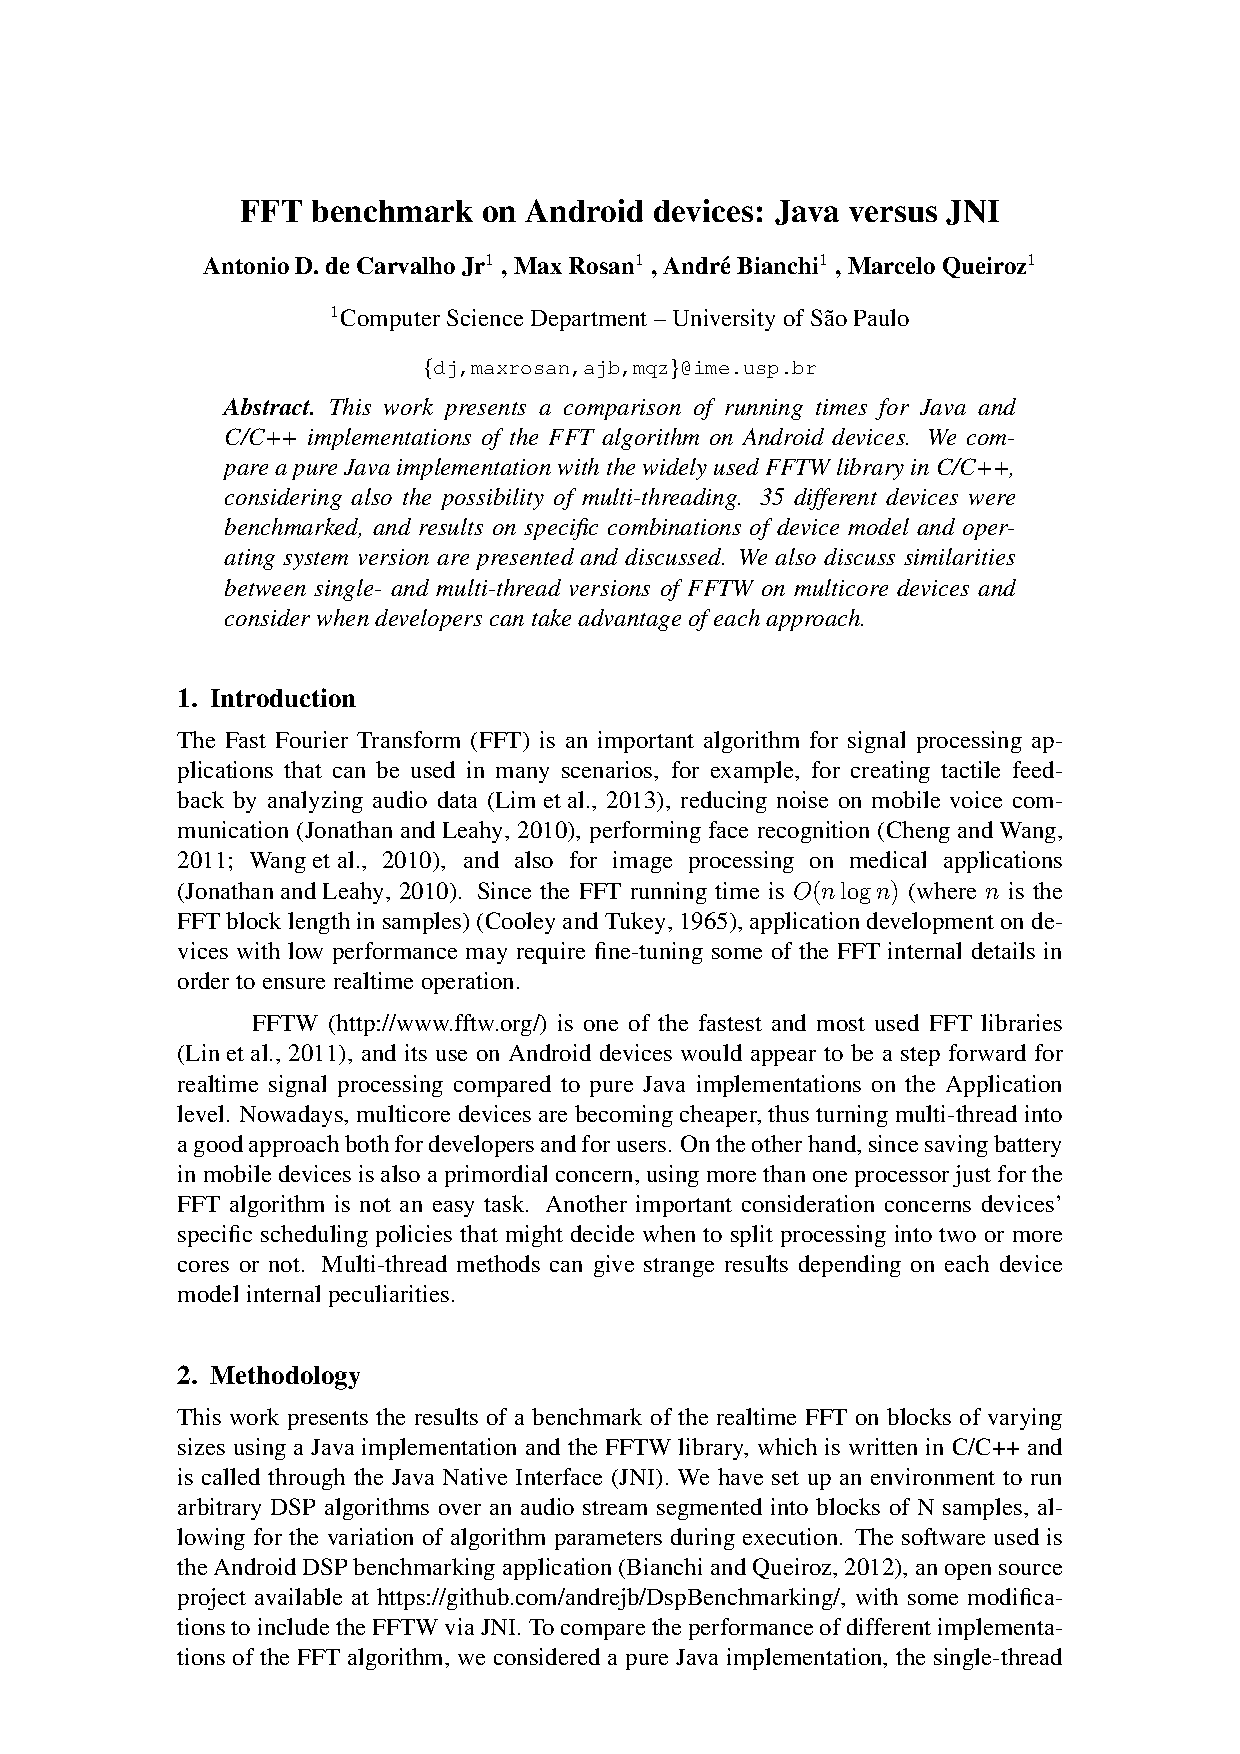
\includepdf[pages=-,frame,scale=0.8,pagecommand={}]{papers/2013-sbcm.pdf}

%% ------------------------------------------------------------------------- %%
\section{ICSC 2013 - Touches on the line: Sharing Csound scores using web server and mobile phones}
\label{ape:papericsc2013}

\subsection*{Paper details}

Title: \textit{Touches on the line: Sharing Csound scores using web server and mobile phones}

Authors: Antonio Deusany de Carvalho Junior

\subsection*{Conference details}

Title: 2nd International CSound Conference~(ICSC)

Venue: Berklee College of Music, Boston, MA, USA

Dates: October 25 to 27, 2013

\subsection*{Remarks}

During the conference, I performed at the Concert \#6 on October 27th with the application running on two mobile devices at the David Friend Recital Hall, Berklee College of Music, Boston, MA, USA~\footnote{\url{http://www.csounds.com/csound-conference-poster-schedule/}}.
This performance happened just before the concert in which performed Jean-Claude Risset, John Chowning, and Richard Boulanger, the masters of Computer Music that I met during this conference.

I also met two important woman for Computer Music during this conference.
Sitting by her side during concerts, I had a brief talk with Marjorie Matthews, the spouse of Max Matthews, the father of Computer Music.
The other woman was Judy Klein, a pianist and professor of electronic music.
We went out for a cup of tea and she exposed me the great history of Computer Music during the 1980's when she was working with the first versions of CSound and waiting the whole night to listen minutes of synthesized sounds.

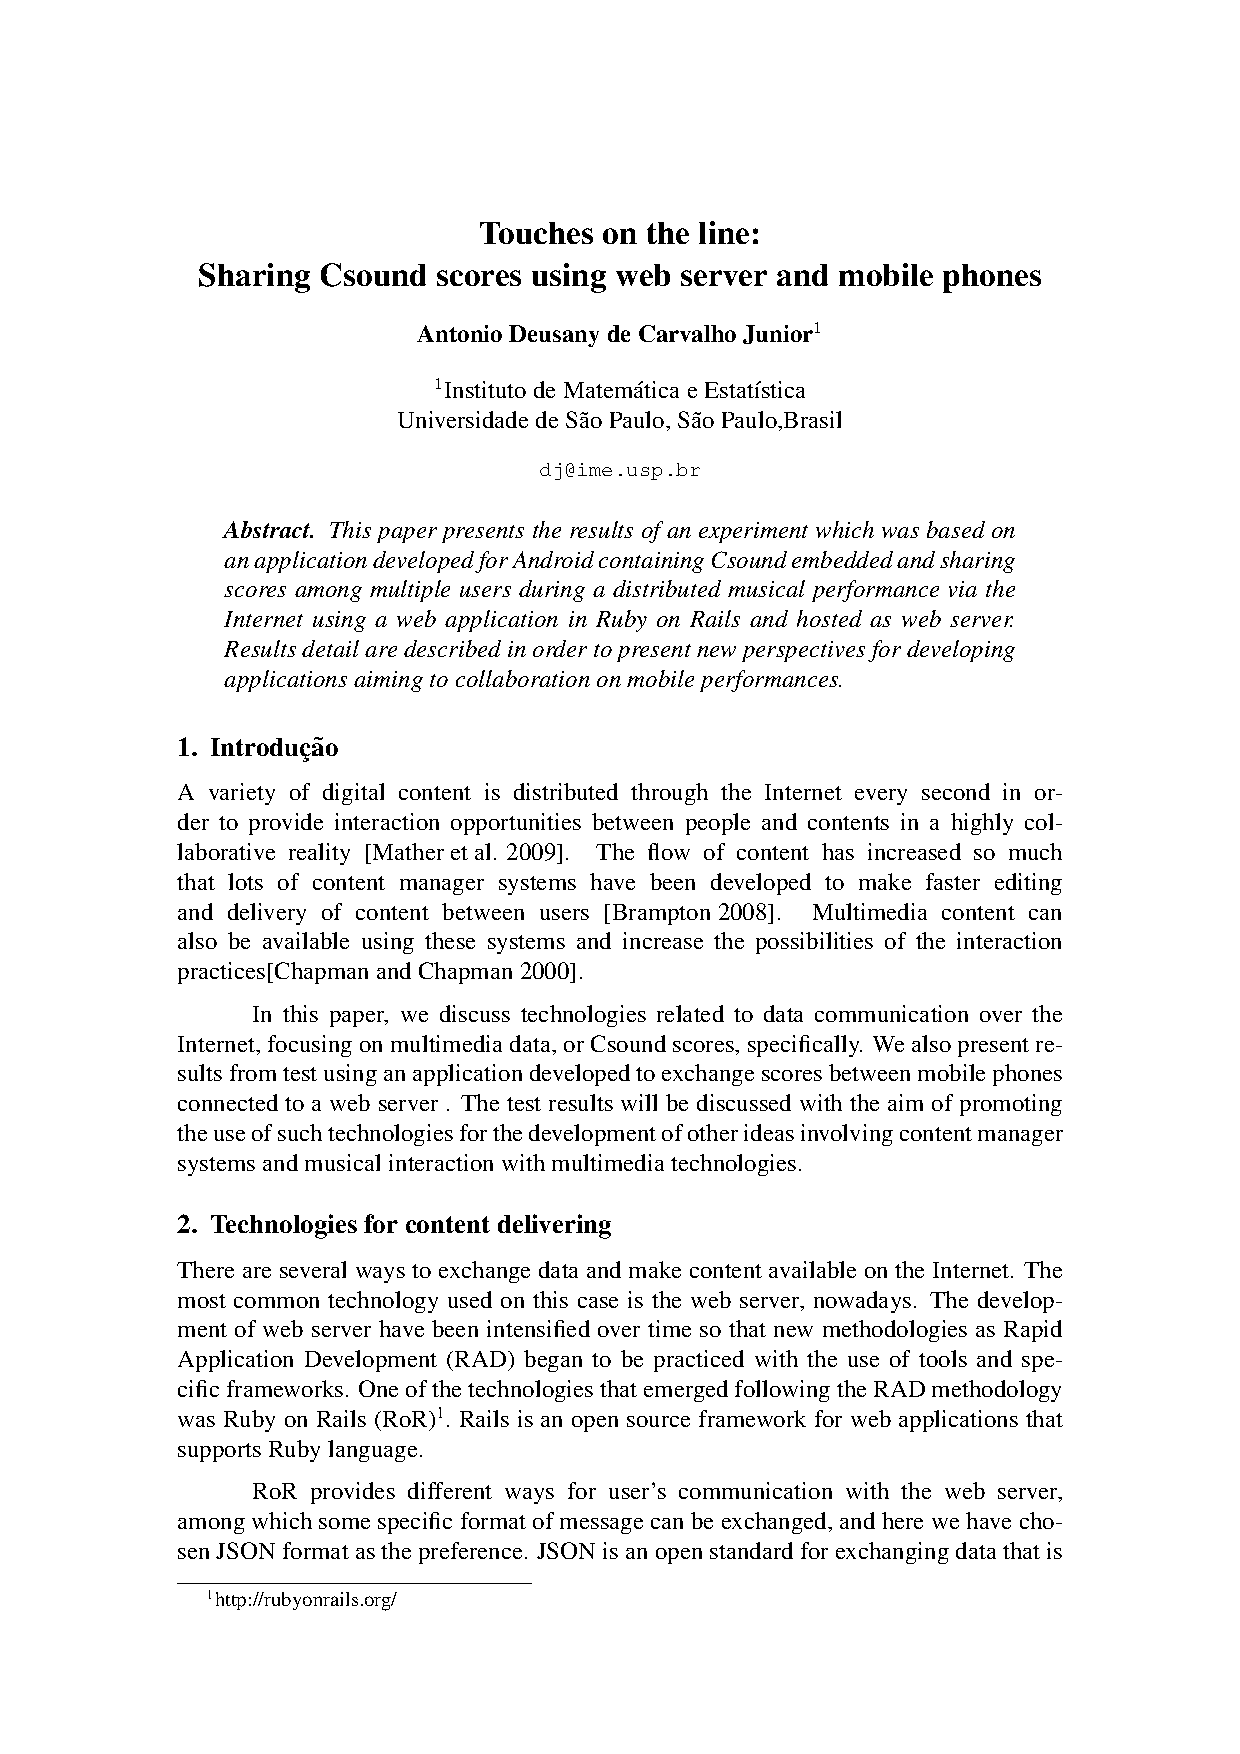
\includepdf[pages=-,frame,scale=0.8,pagecommand={}]{papers/2013-csound.pdf}

%% ------------------------------------------------------------------------- %%
\section{BATS 2014 - Notes on the Elimination of the Mobile Music Audience}
\label{ape:paperbats2014}

\subsection*{Paper details}

Title: \textit{Notes on the Elimination of the Mobile Music Audience}

Authors: André Damião Bandeira, Antonio Deusany de Carvalho Junior

\subsection*{Conference details}

Title: 14th Biennial Arts and Technology Symposium

Venue: Connecticut College, Ammerman Center for Arts and Technology, New London, CT

Dates: February 27, 28 and March 1, 2014

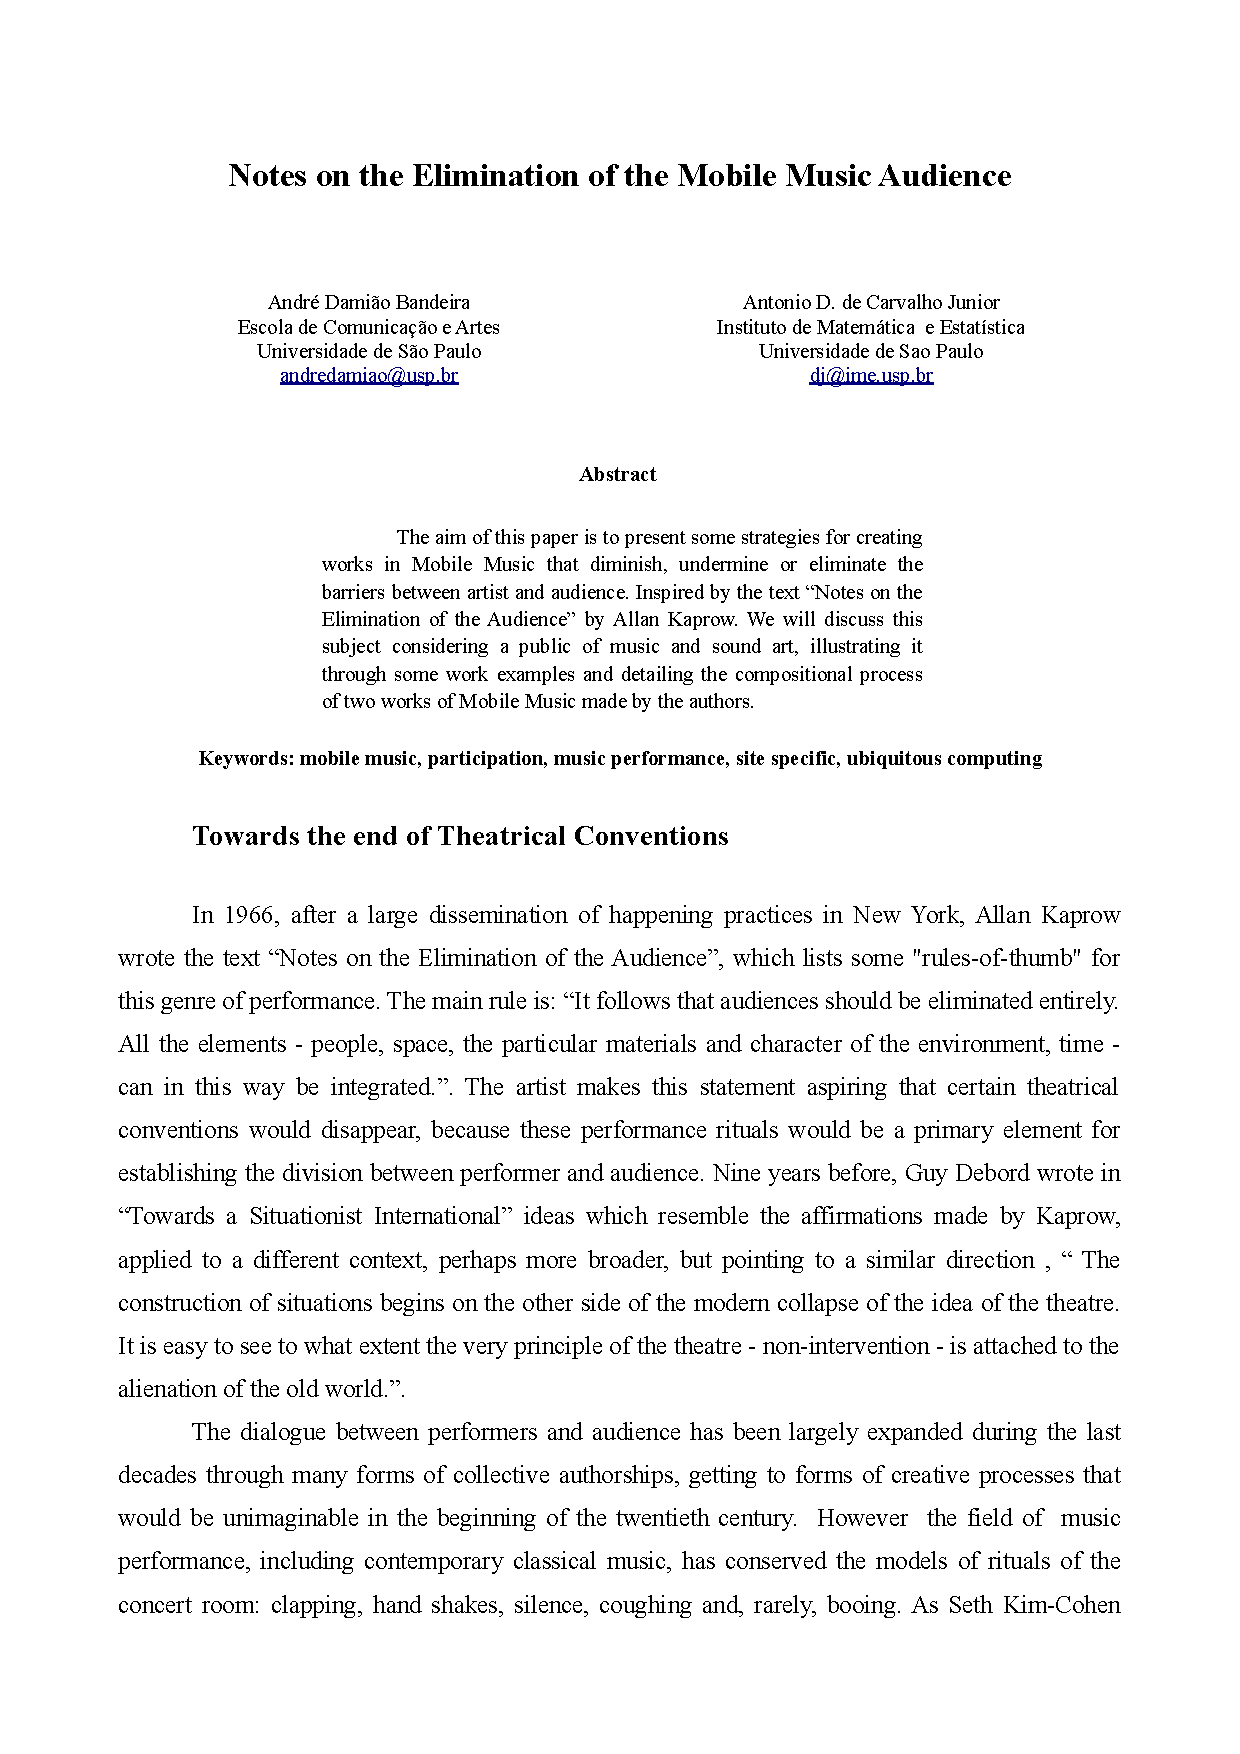
\includepdf[pages=-,frame,scale=0.8,pagecommand={}]{papers/2014-bienial-compressed.pdf}

%% ------------------------------------------------------------------------- %%
\section{ICMC 2014 - Sensors2PD: Mobile sensors and WiFi information as input for Pure Data}
\label{ape:papericmc2014}

\subsection*{Paper details}

Title: \textit{Sensors2PD: Mobile sensors and WiFi information as input for Pure Data}

Authors: Antonio Deusany de Carvalho Junior

\subsection*{Conference details}

Title: 40th International Computer Music Conference and 11th Sound and Music Computing Conference

Venue: Athens, Greece

Dates: September 14 to 20, 2014 

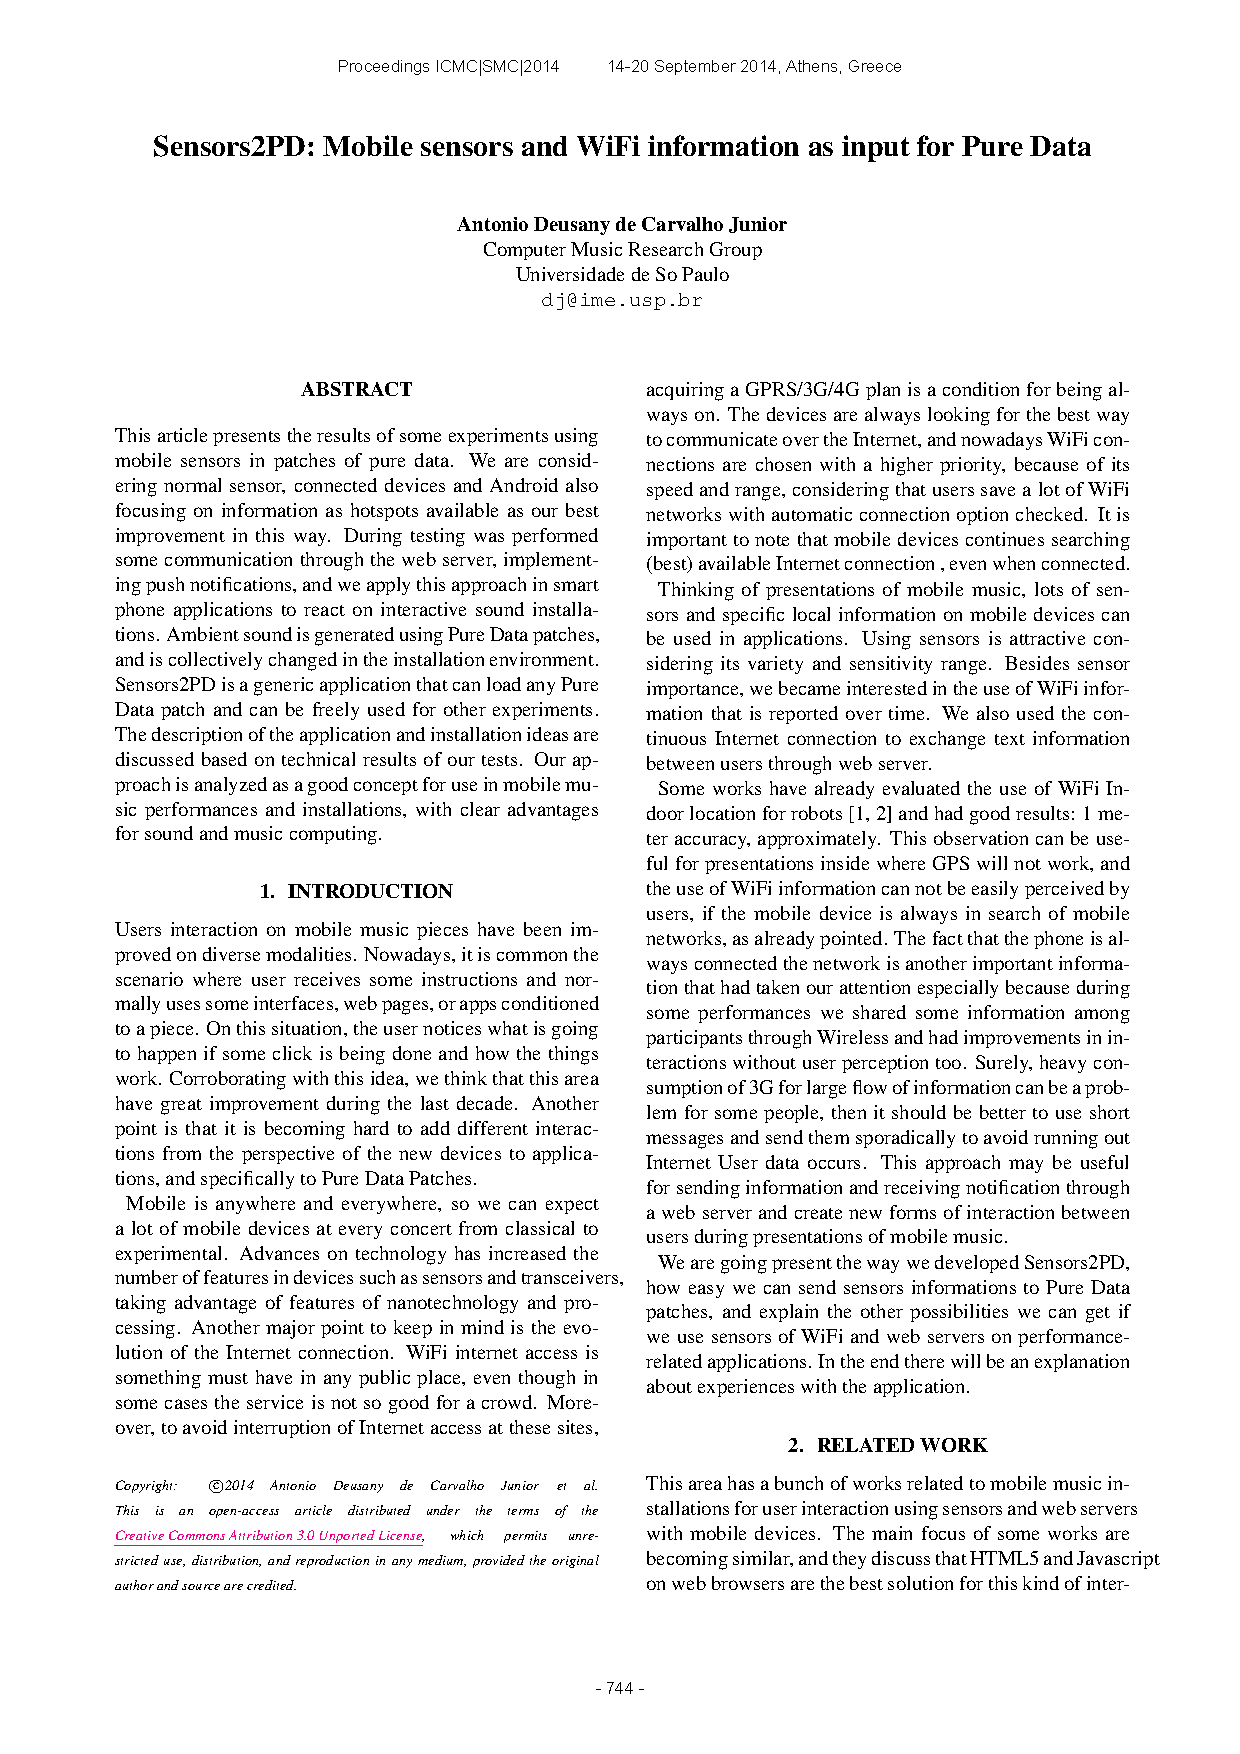
\includepdf[pages=-,frame,scale=0.8,pagecommand={}]{papers/2014-icmcsmc.pdf}

%% ------------------------------------------------------------------------- %%
\section{NIME 2015 - Indoor localization during installations using Wi-Fi}
\label{ape:papernime2015}

\subsection*{Paper details}

Title: \textit{Indoor localization during installations using Wi-Fi}

Authors: Antonio Deusany de Carvalho Junior

\subsection*{Conference details}

Title: 15th International Conference on New Interfaces for Musical Expression

Venue: Lousiana State University, Banton Rouge, LA, USA

Dates: May 31 to June 3, 2015

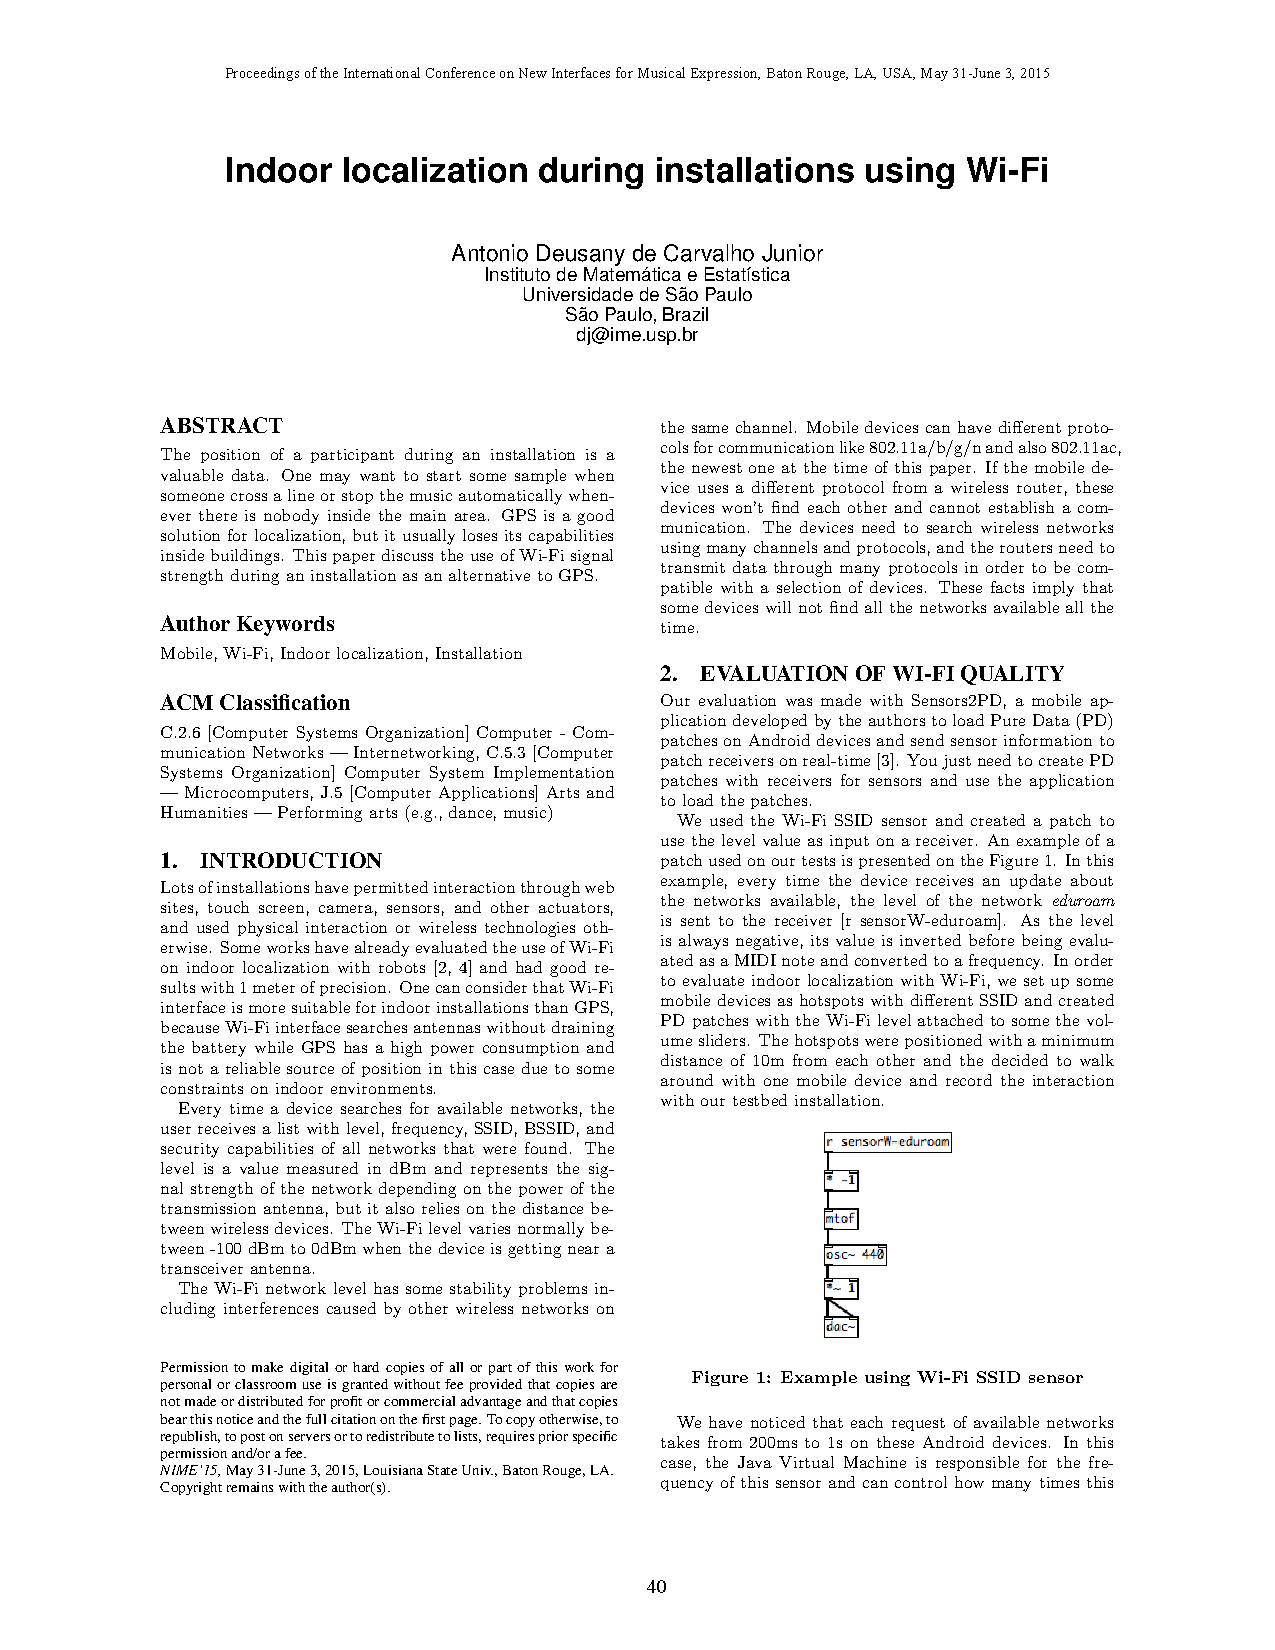
\includepdf[pages=-,frame,scale=0.8,pagecommand={}]{papers/2015-nime.pdf}

%% ------------------------------------------------------------------------- %%
\section{SMC 2015 - Sensors2OSC}
\label{ape:papersmc2015}

\subsection*{Paper details}

Title: \textit{Sensors2OSC}

Authors: Antonio Deusany de Carvalho Junior, Thomas Mayer

\subsection*{Conference details}

Title: 12th Sound and Music Computing Conference

Venue: Maynooth University, Ireland

Dates: July 26 to August 1, 2015

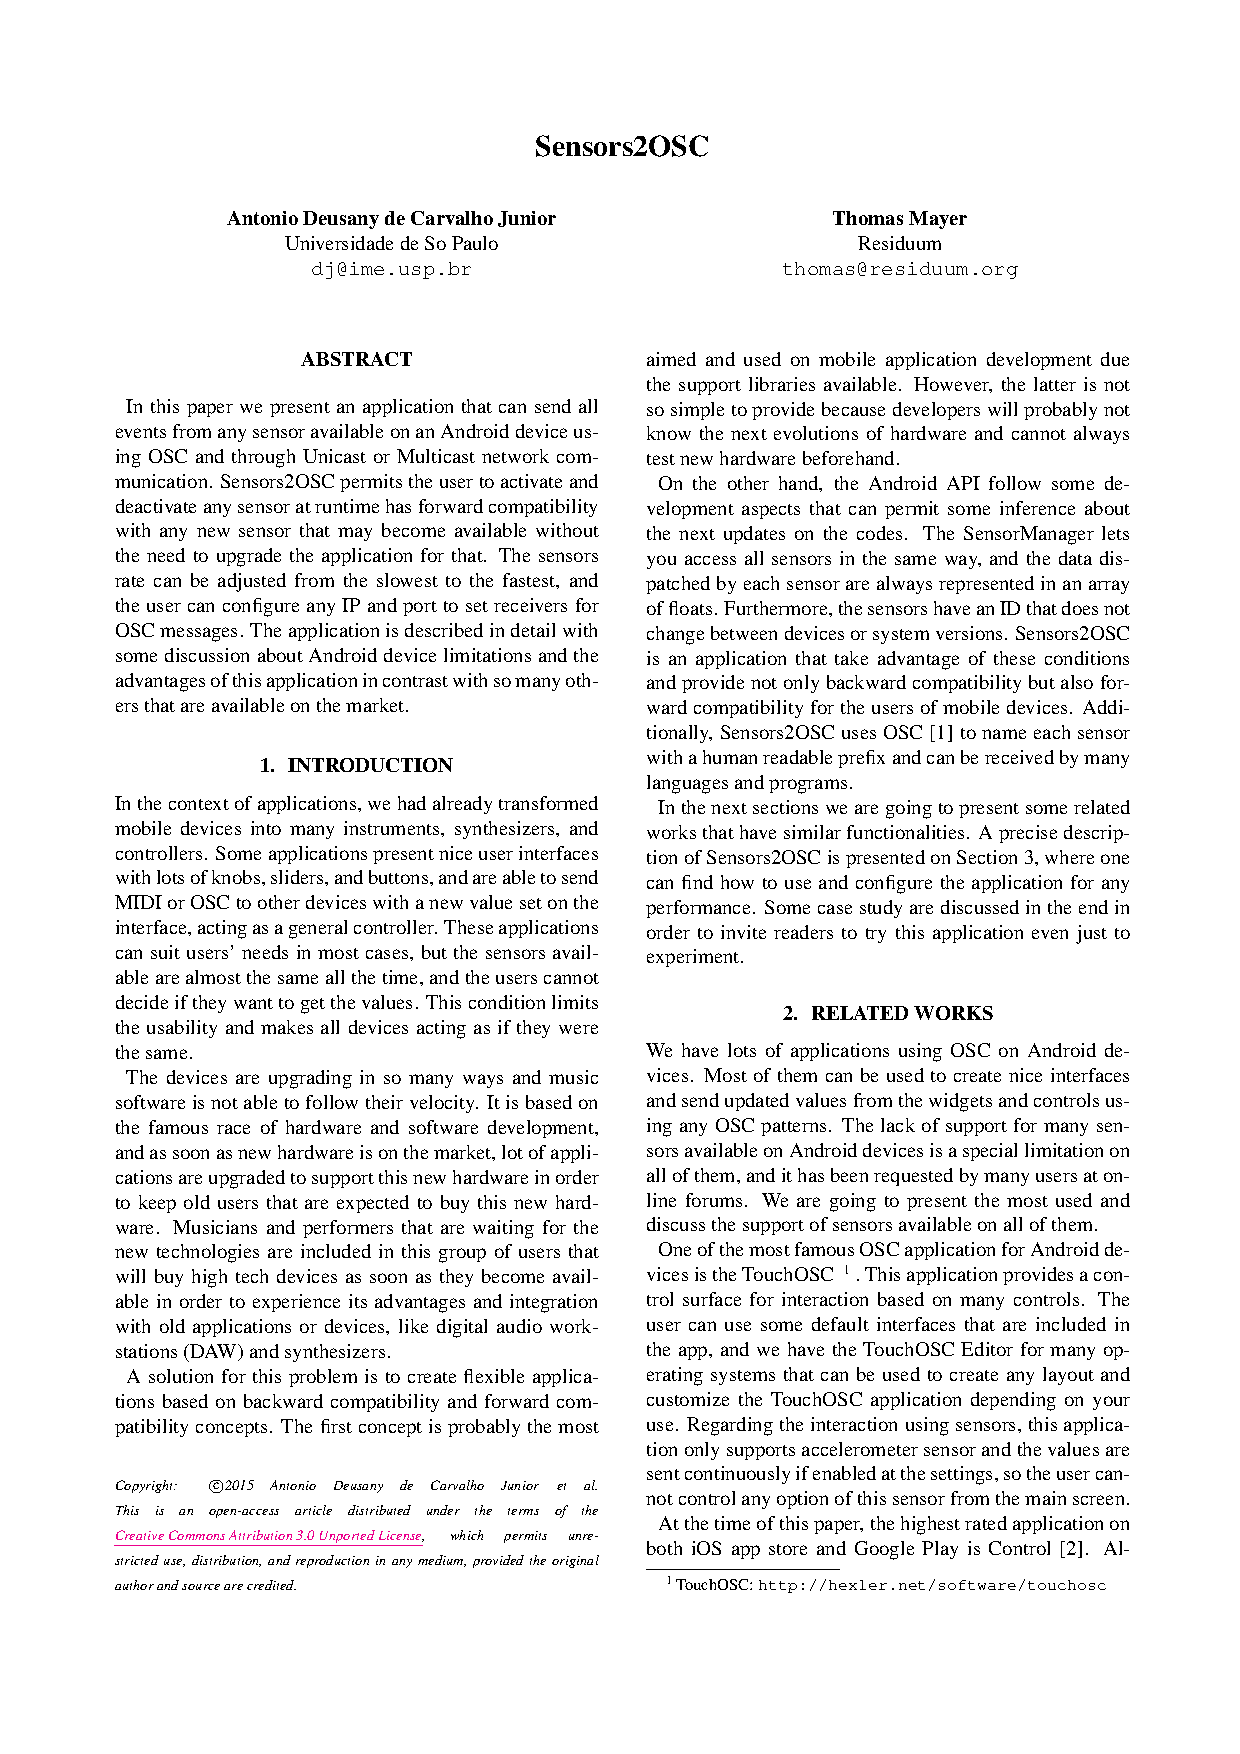
\includepdf[pages=-,frame,scale=0.8,pagecommand={}]{papers/2015-smc.pdf}

%% ------------------------------------------------------------------------- %%
\section{ICMC 2015 - Computer Music through the Cloud: Evaluating a Cloud Service for Collaborative Computer Music Applications}
\label{ape:papericmc2015}

\subsection*{Paper details}

Title: \textit{Computer Music through the Cloud: Evaluating a Cloud Service for Collaborative Computer Music Applications}

Authors: Antonio Deusany de Carvalho Junior, Marcelo Queiroz, Georg Essl

\subsection*{Conference details}

Title: 41st International Computer Music Conference~(ICMC)

Venue: University of North Texas, Denton, TX, USA

Dates: September 25 to October 1, 2015

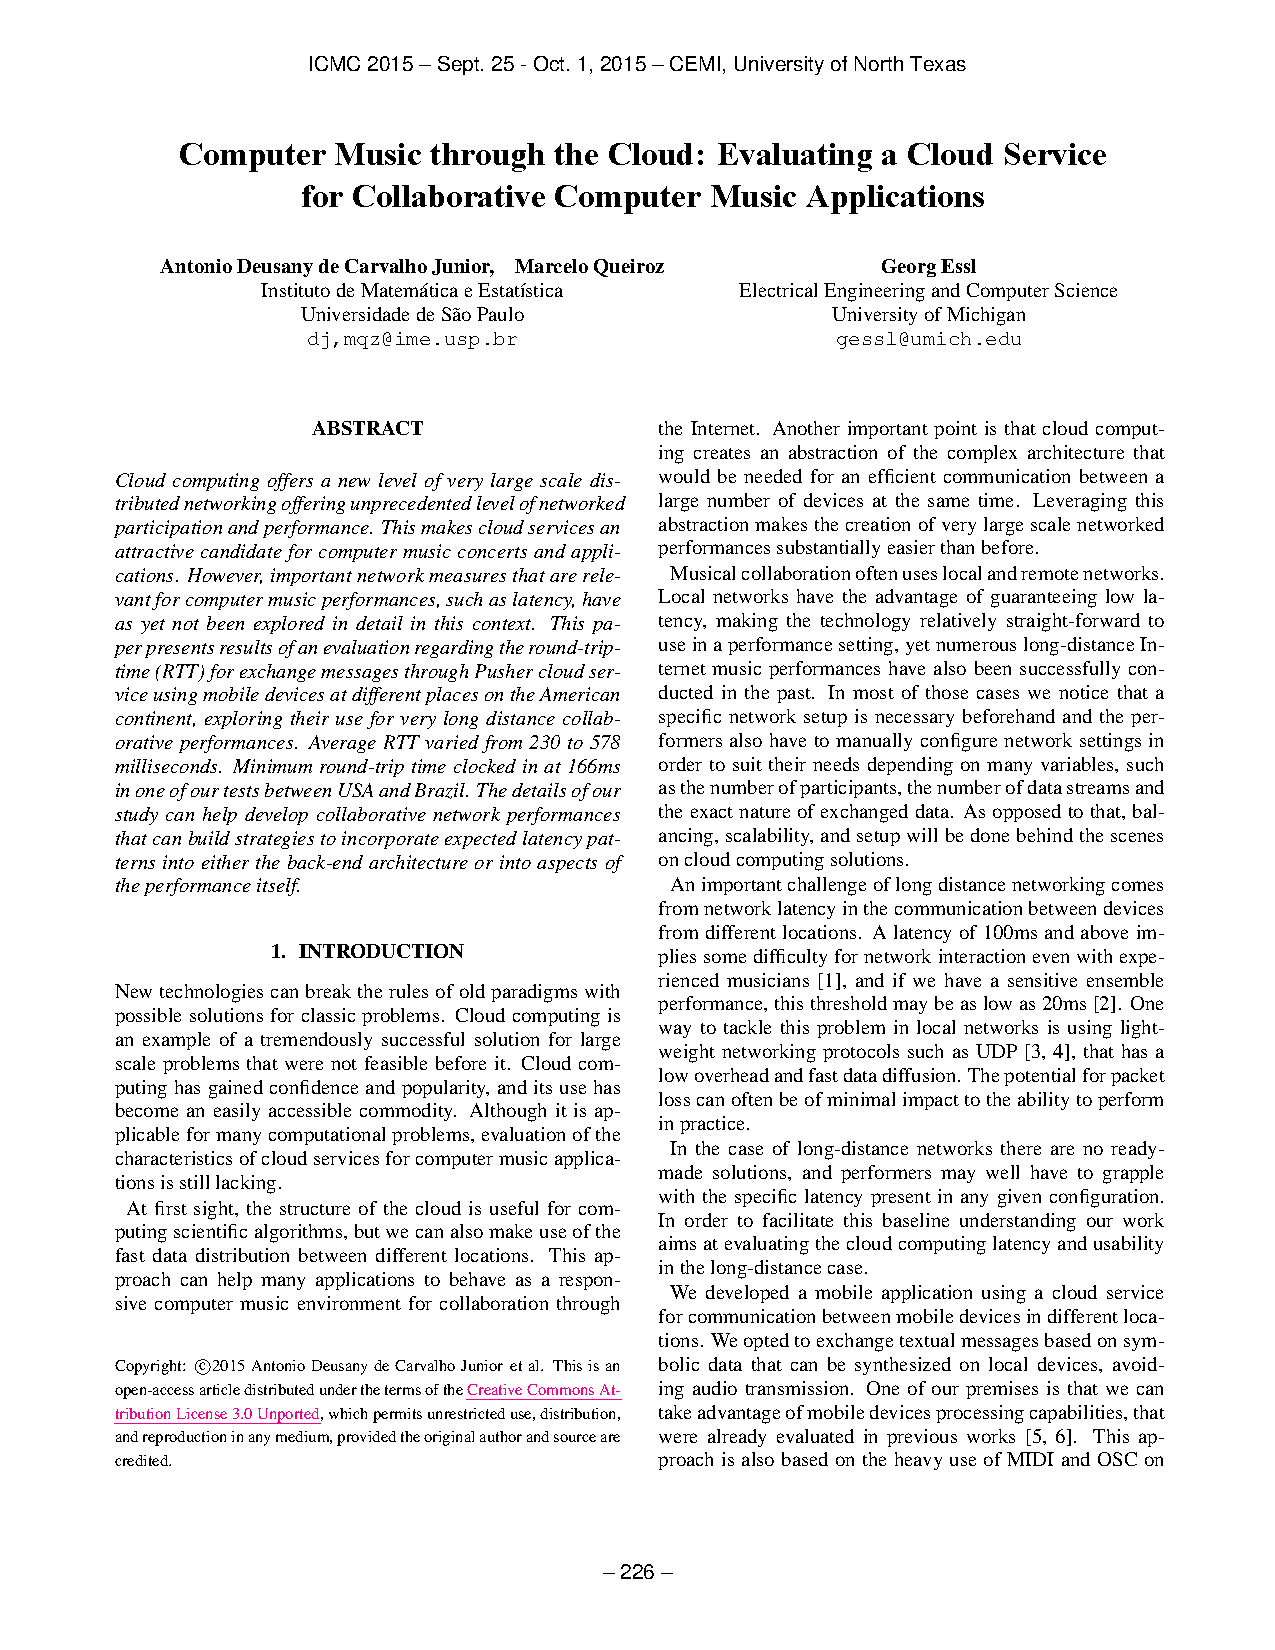
\includepdf[pages=-,frame,scale=0.8,pagecommand={}]{papers/2015-icmc.pdf}

%% ------------------------------------------------------------------------- %%
\section{ICLC 2015 - SuperCopair: Collaborative Live Coding on SuperCollider through the cloud}
\label{ape:papericlc2015}

\subsection*{Paper details}

Title: \textit{SuperCopair: Collaborative Live Coding on SuperCollider through the cloud}

Authors: Antonio Deusany de Carvalho Junior, Sang Won Lee, Georg Essl

\subsection*{Conference details}

Title: International Conference on Live Coding~(ICLC)

Venue: School of Music, University of Leeds, UK

Dates: July 13 to 15, 2015

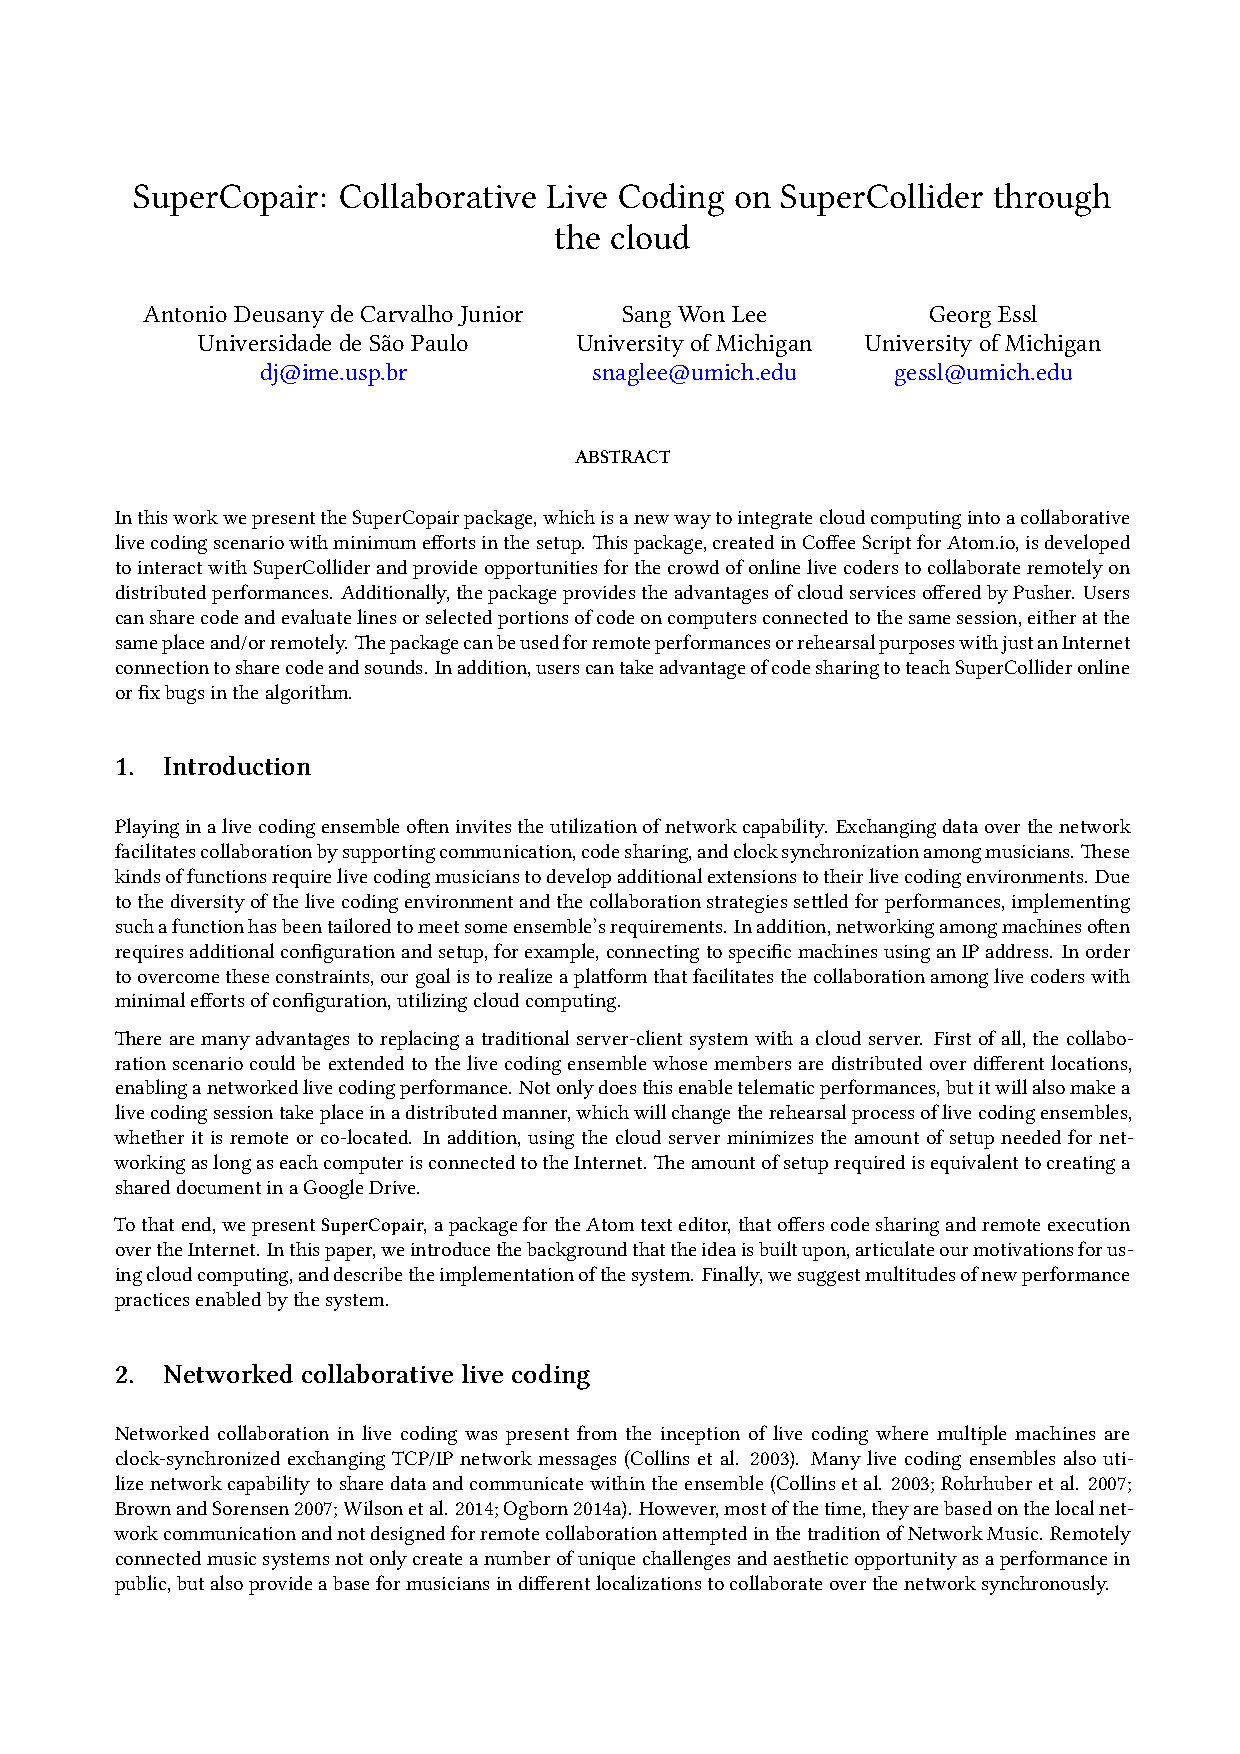
\includepdf[pages=-,frame,scale=0.8,pagecommand={}]{papers/2015-iclc.pdf}

%% ------------------------------------------------------------------------- %%
\section{CLEI 2015 - Cooperative Live Coding as an instructional model}
\label{ape:paperclei2015}

\subsection*{Paper details}

Title: \textit{Cooperative Live Coding as an instructional model}

Authors: Antonio Deusany de Carvalho Junior

\subsection*{Conference details}

Title: XLI Conferencia Latinoamericana en Informática~(CLEI)

Venue: Arequipa, Peru

Dates: October 19 to 23, 2015

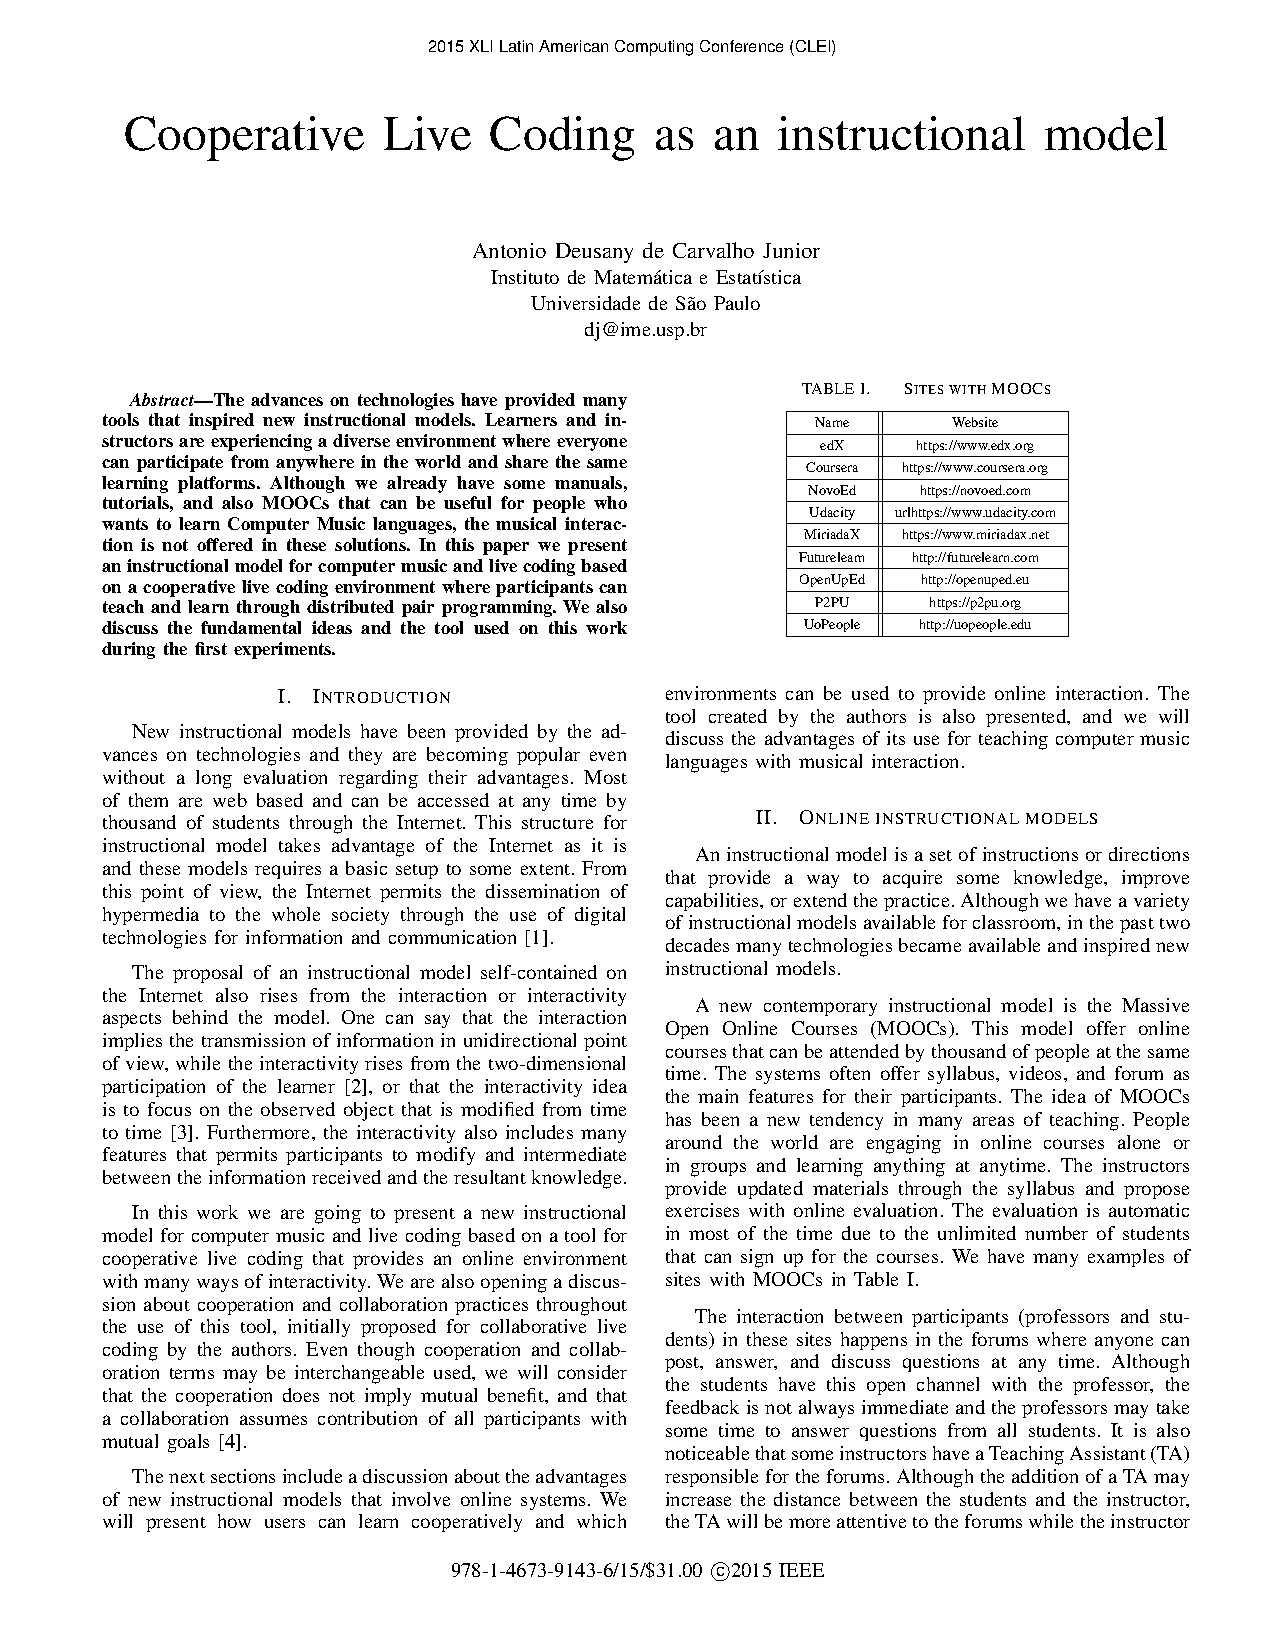
\includepdf[pages=-,frame,scale=0.8,pagecommand={}]{papers/2015-clei.pdf}

%% ------------------------------------------------------------------------- %%
\section{WAC 2016 - Crowd in C[loud]: Audience Participation Music with Online Dating Metaphor using Cloud Service}
\label{ape:paperwac2016}

\subsection*{Paper details}

Title: \textit{Crowd in C[loud]: Audience Participation Music with Online Dating Metaphor using Cloud Service}

Authors: Sang Won Lee, Antonio Deusany de Carvalho Junior, Georg Essl

\subsection*{Conference details}

Title: 2nd Web Audio Conference~(WAC)

Venue: Georgia Tech, Atlanta, GA, USA

Dates: April 4 to 6, 2016

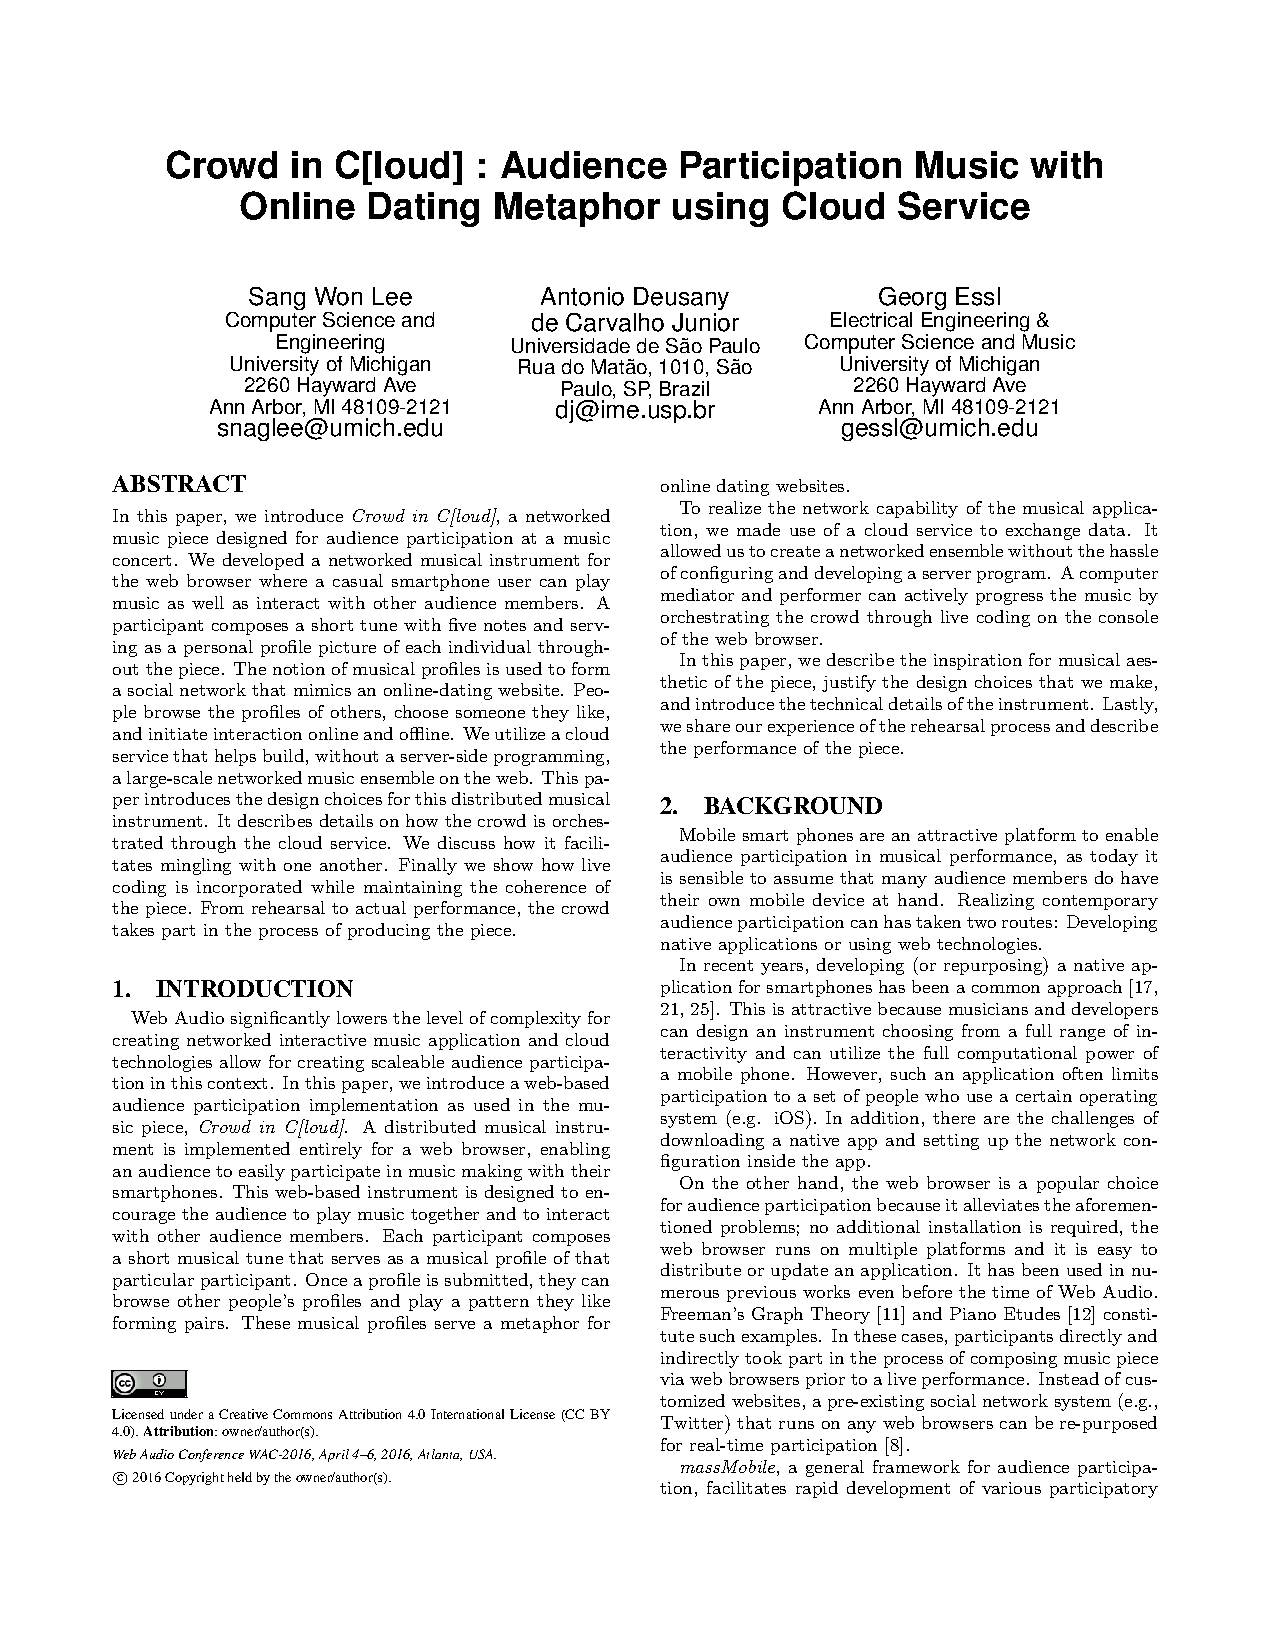
\includepdf[pages=-,frame,scale=0.8,pagecommand={}]{papers/2016-webaudio.pdf}

%% ------------------------------------------------------------------------- %%
\section{NIME 2016 - Understanding Cloud Service in the Audience Music Performance of Crowd in C[loud]}
\label{ape:papernime2016}

\subsection*{Paper details}

Title: \textit{Understanding Cloud Service in the Audience Music Performance of Crowd in C[loud]}

Authors: Antonio Deusany de Carvalho Junior, Sang Won Lee, Georg Essl

\subsection*{Conference details}

Title: 16th International Conference on New Interfaces for Musical Expression

Venue: Griffith University, Brisbane, Australia

Dates: July 11 to 15, 2016

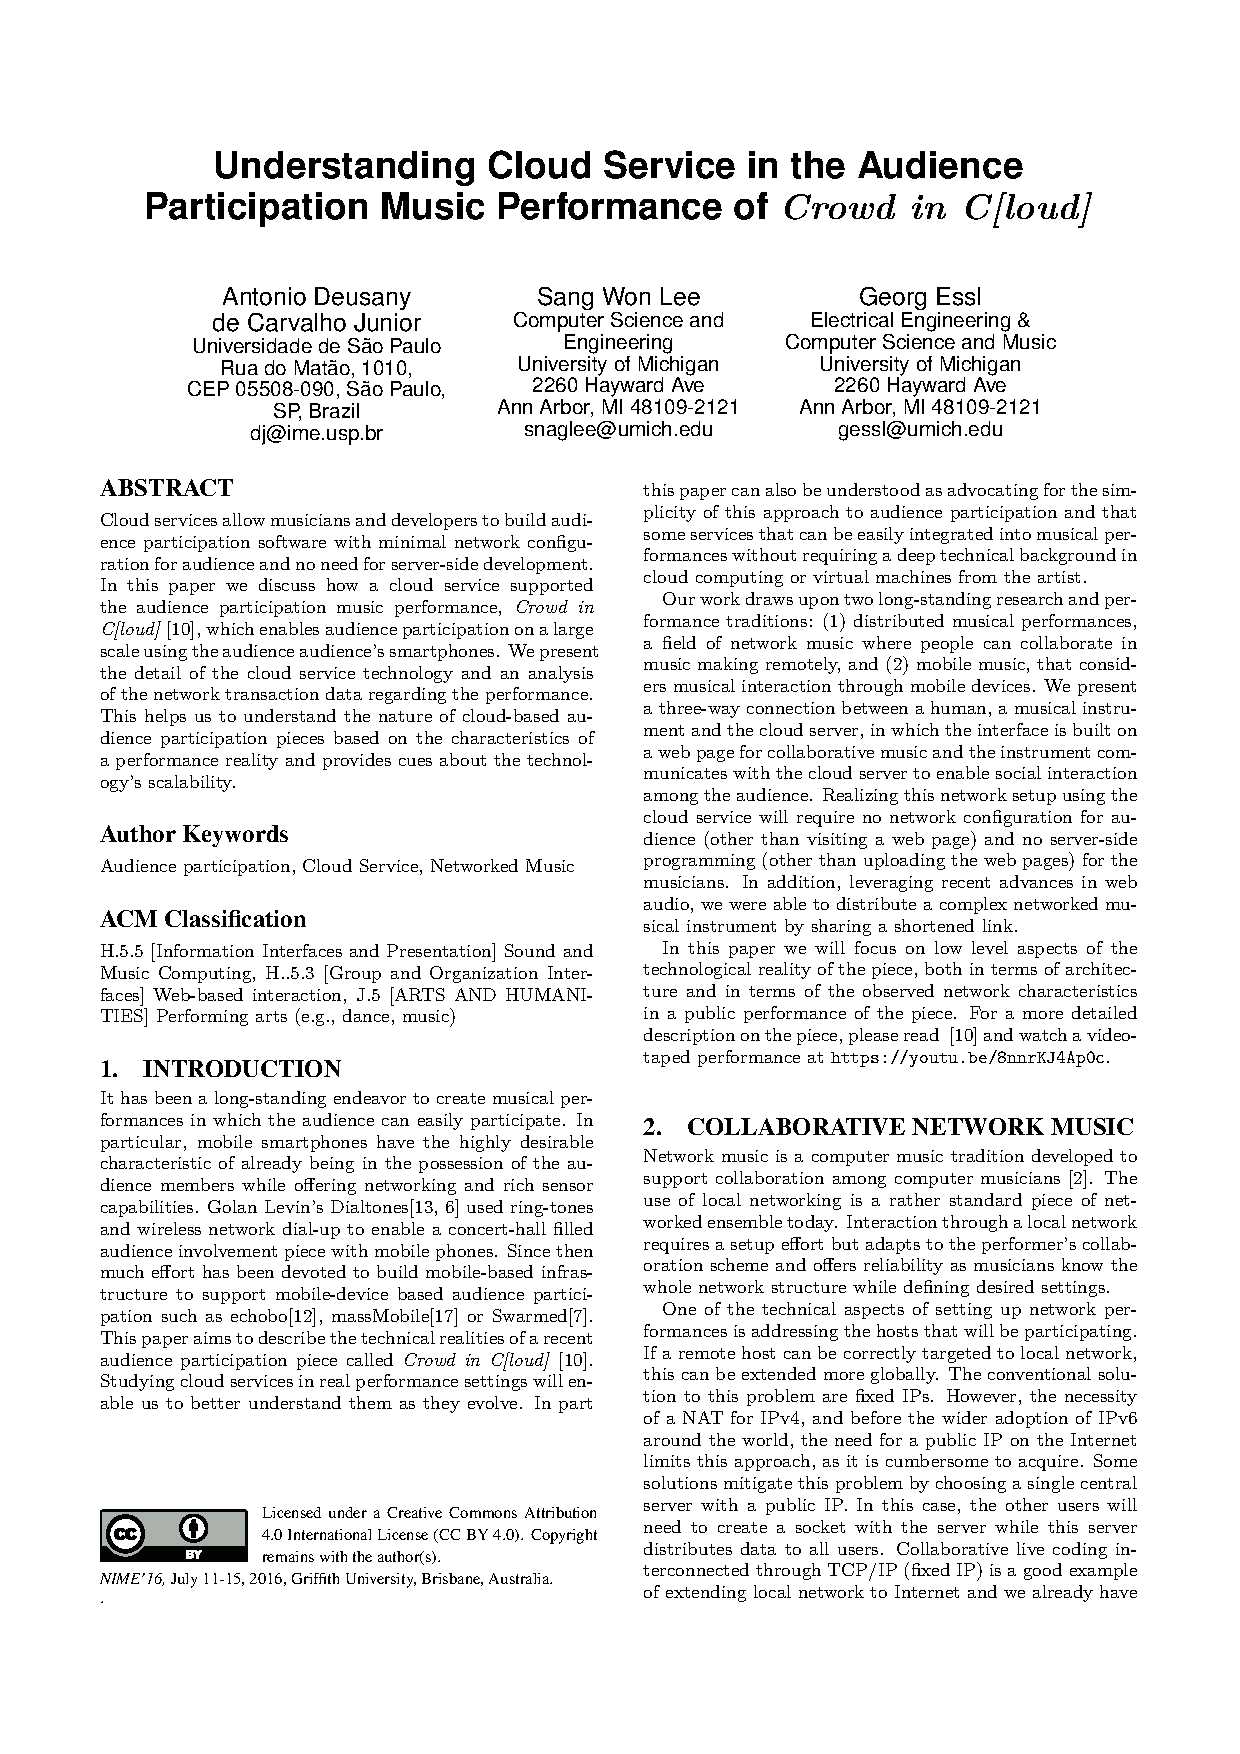
\includepdf[pages=-,frame,scale=0.8,pagecommand={}]{papers/2016-nime.pdf}

%% ------------------------------------------------------------------------- %%
\section{WAC 2017 - Open band: Audience Creative Participation Using Audio Synthesis}
\label{ape:paperwac2017}

\subsection*{Paper details}

Title: \textit{Open band: Audience Creative Participation Using Audio Synthesis}

Authors: Ariane Stolfi, Fábio Goródscy, Antonio Deusany de Carvalho Junior, Fernando Iazzetta, Mathieu Barthet

\subsection*{Conference details}

Title: 3rd Web Audio Conference~(WAC)

Venue: Centre for Digital Music, Queen Mary University of London, London, UK

Dates: August 21 to 23, 2017

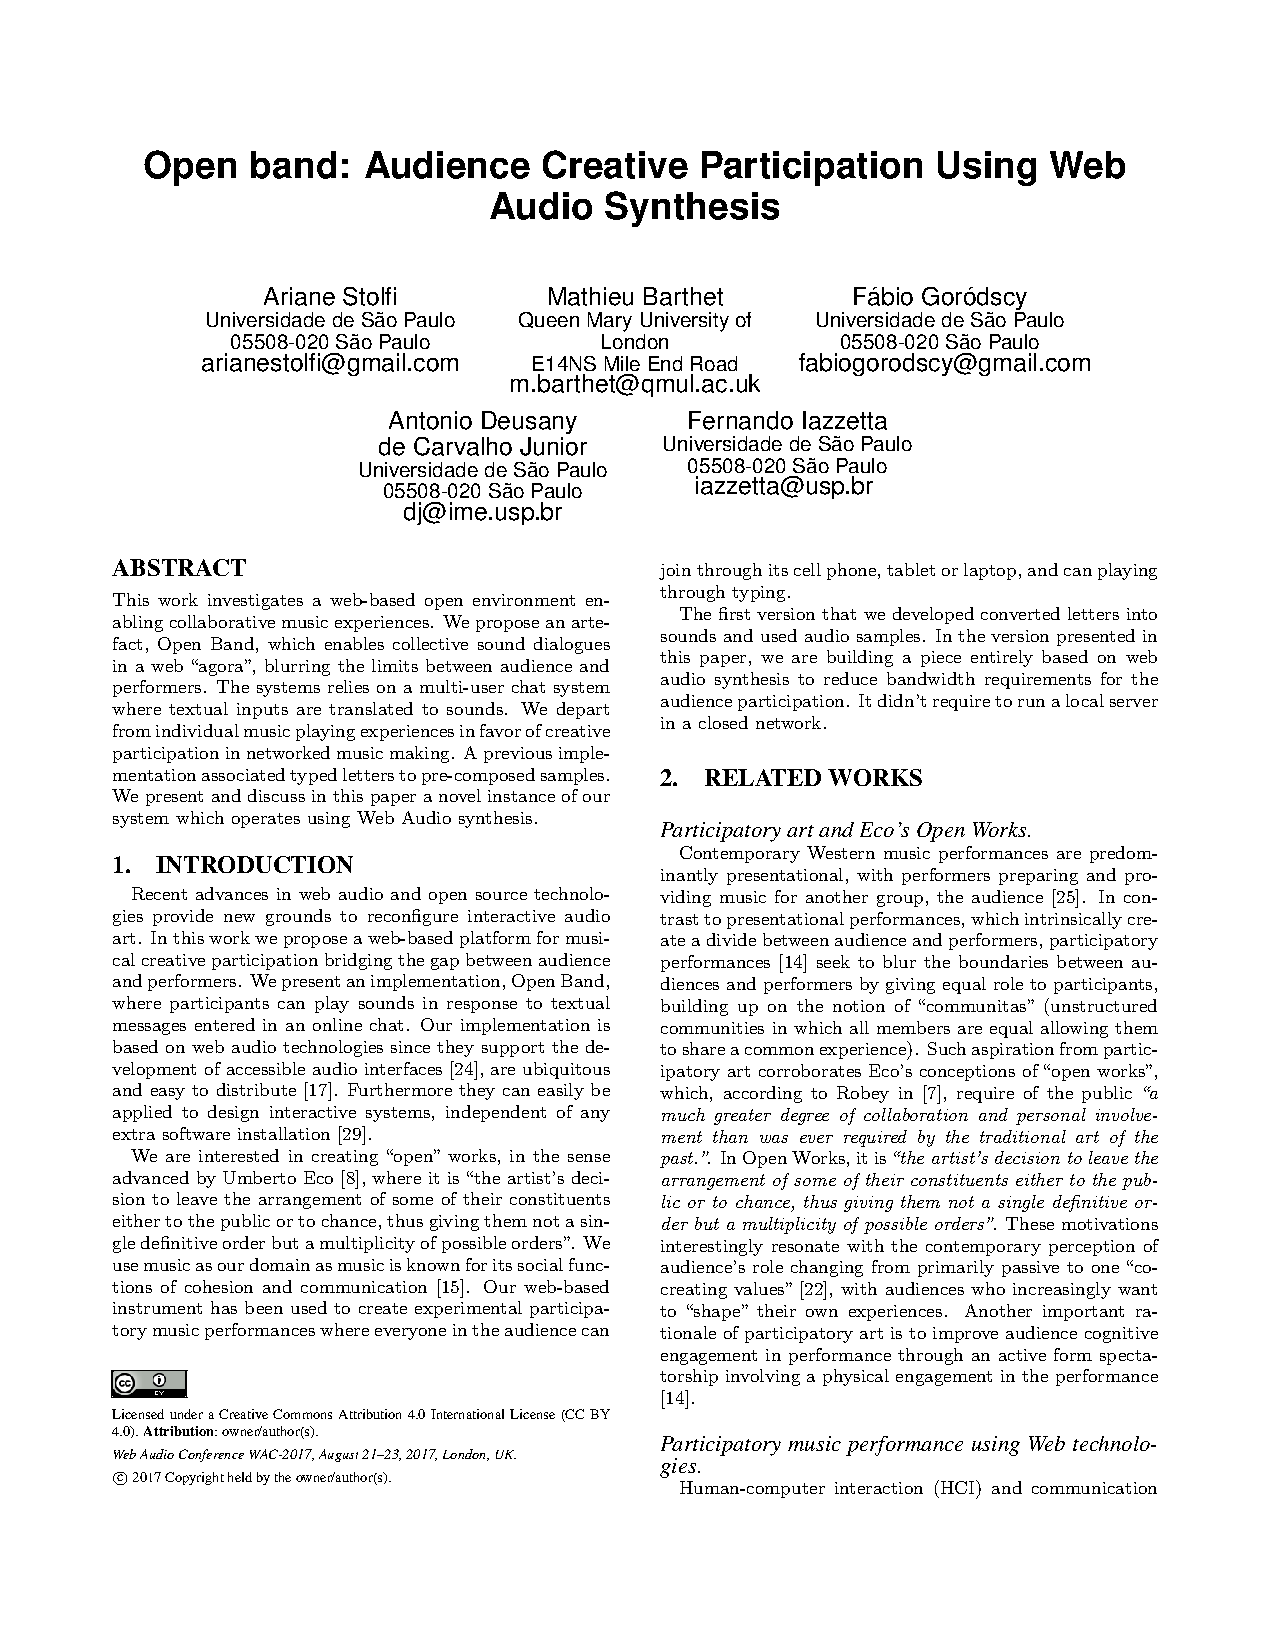
\includepdf[pages=-,frame,scale=0.8,pagecommand={}]{papers/2017-webaudio.pdf}

%% ------------------------------------------------------------------------- %%
\section{Audio Mostly 2017 - Open Band: A Platform for Collective Sound Dialogues}
\label{ape:paperam2017}

\subsection*{Paper details}

Title: \textit{Open band: A Platform for Collective Sound Dialogues}

Authors: Ariane Stolfi, Fábio Goródscy, Antonio Deusany de Carvalho Junior, Mathieu Barthet

\subsection*{Conference details}

Title: Audio Mostly

Venue: Centre for Digital Music, Queen Mary University of London, London, UK
 
Dates: August 23 to 26, 2017

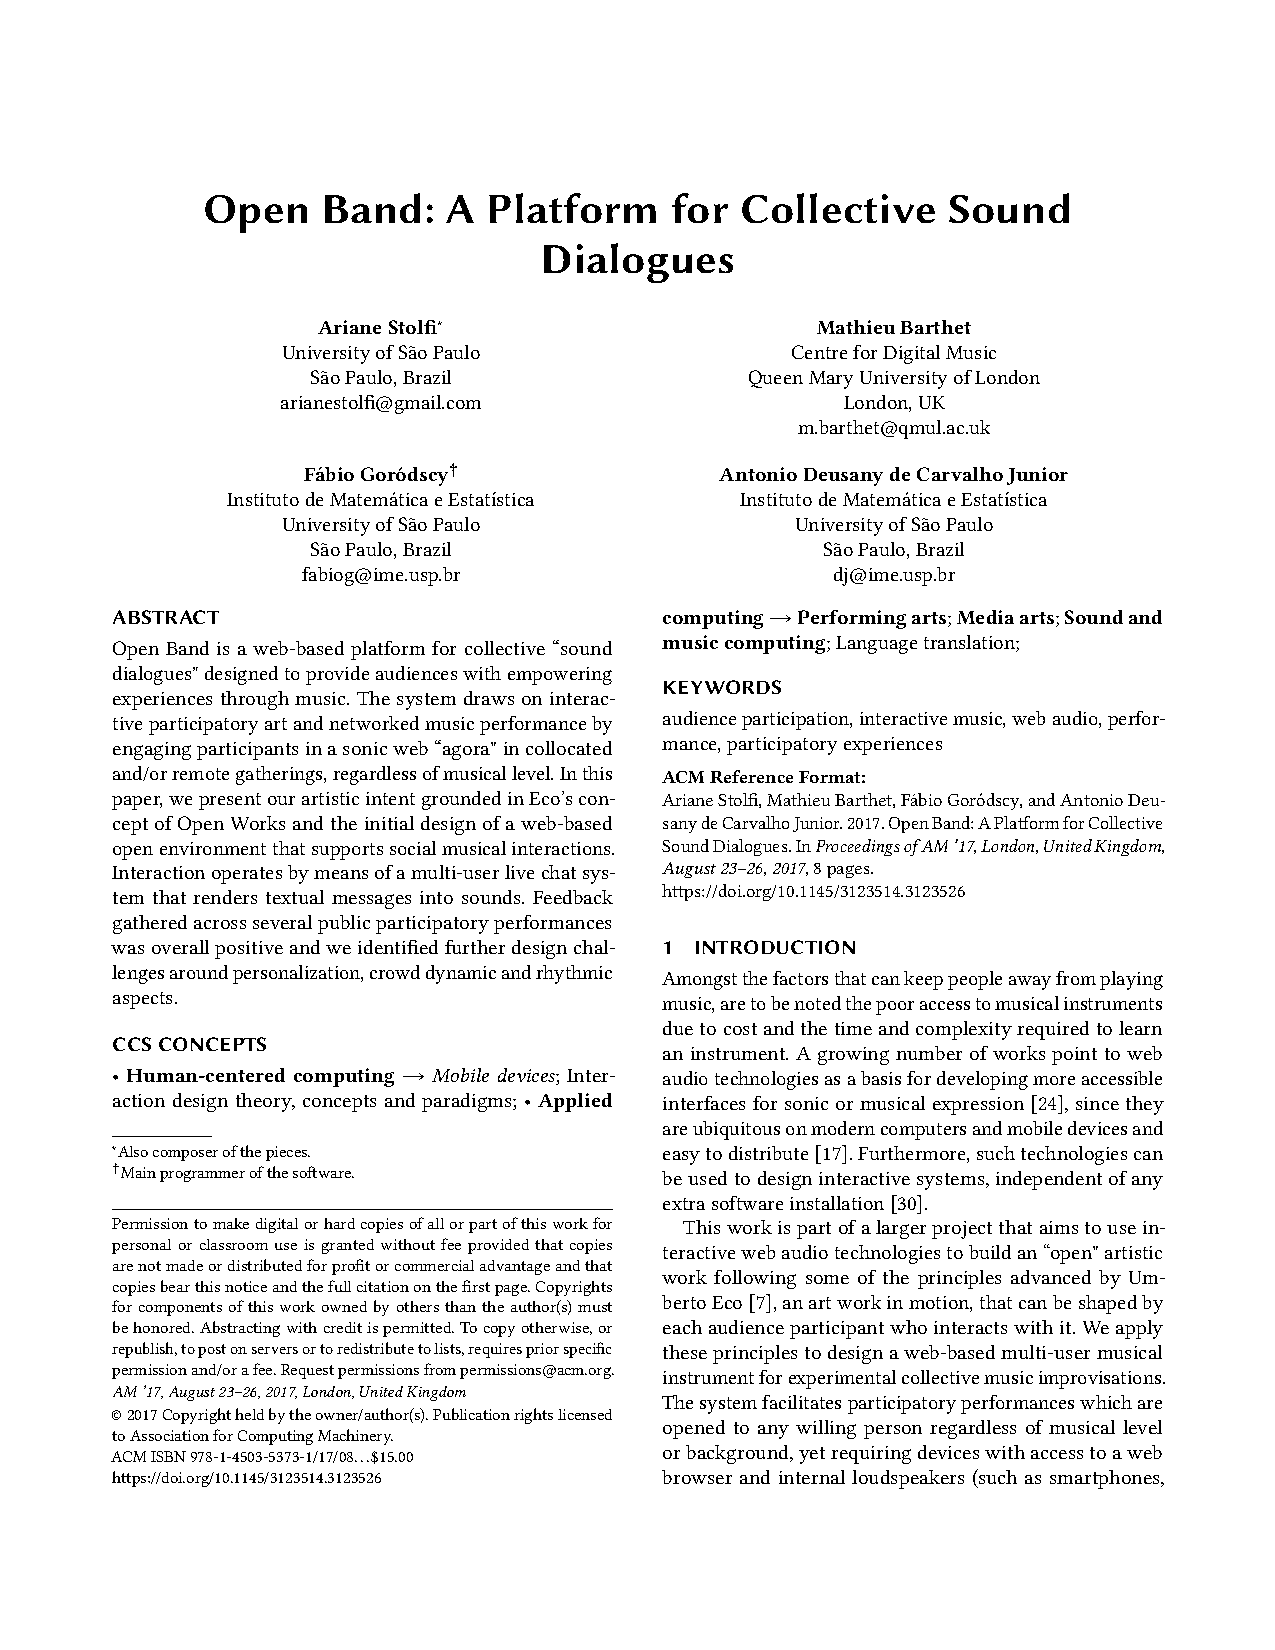
\includepdf[pages=-,frame,scale=0.8,pagecommand={}]{papers/2017-audiomostly.pdf}
